%%%%%%%%%%%%%%%
% This style of this thesis is based on the thesis proposal required to be submitted at the start of the Master's thesis project in the Artificial Intelligence program.
% It has been updated with the new high-res banner for the Faculty of Science and Engineering, and includes, among other features, a contents page, an acknowledgements page, and appendices.

% Author: Manvi Agarwal
% Last modified: 15 December 2020
%%%%%%%%%%%%%%%



\documentclass[a4paper,12pt,twoside]{article}
%\documentclass[a4paper,12pt]{article}
\usepackage{comment}
\usepackage{lipsum}
\usepackage{multirow}
\usepackage{subcaption}
\usepackage{xcolor}
\usepackage{amsmath}
\usepackage{amssymb}   % \mathbb, \mathcal and math symbols
\usepackage{amsfonts}
\usepackage{wrapfig}    % inline figures
\usepackage{enumitem}
\usepackage{mwe}
\usepackage{graphicx} % Use for Images
\graphicspath{{images/}}
\usepackage{pdflscape} % Full-page landscape tables (rotates the PDF page)
\usepackage{here}     % Forced Figure Placement
% NOTE: pslatex/mathptmx require the rsfs script font for \mathcal, which is
% not available in this TeX install; using default Computer Modern fonts.
\usepackage{fancyhdr} % Use headers
\usepackage{float}
\usepackage{placeins}        % \FloatBarrier to flush pending floats
\usepackage{titlesec}        % section heading spacing control
\usepackage{algorithm}       % pseudocode float
\usepackage{algpseudocode}   % pseudocode body (algorithmicx)
% Here I keep the left and right margins equal. You can choose to have unequal margins if you want a two-sided book effect.
\usepackage[
	top    = 1.5cm,
	bottom = 1.80cm,
	left   = 2.00cm,
	right  = 2.00cm,
	includeheadfoot]{geometry} % Use similar margins to the Word Template
\setlength{\parindent}{0pt}

% Tighten run-in \paragraph spacing (default 3.25ex -> 1ex before-skip)
\titlespacing{\paragraph}{0pt}{1ex plus 0.5ex minus 0.2ex}{0.5em}

% Placeholder for results pending from the running HPC experiment set.
% \TBD prints a red "TBD" token; results filled in once the experiment set completes.
\newcommand{\TBD}{\textcolor{red}{\textbf{TBD}}}

% Visible red flag for content still supported only by the OLD single-seed
% results, to be replaced once the new experiment set completes.
\newcommand{\oldresults}[1]{%
  \par\smallskip\noindent\textcolor{red}{\rule{\linewidth}{0.6pt}}\par\nobreak
  \noindent\textcolor{red}{\textbf{OLD RESULTS --- pending experiment set: #1}}\par\nobreak
  \noindent\textcolor{red}{\rule{\linewidth}{0.6pt}}\par\smallskip}
% Inline red flag for a single old-results claim.
\newcommand{\oldflag}[1]{\textcolor{red}{#1}}

% Define the page styles
\fancypagestyle{titlepage}{
	\fancyhf{}
	\fancyhead[C]{
\includegraphics[width=\textwidth]{images/banner.png}}
	\renewcommand{\headrulewidth}{0pt}
}

%\fancypagestyle{body}{
%	\fancyhf{}
%  \fancyhead[C]{
\includegraphics{images/banner.png}}
%}

\fancypagestyle{body}{
    \fancyhf{}
    \fancyhead[LE,RO]{\thepage}
    \fancyhead[RE,LO]{Chapter \leftmark}
}



\fancypagestyle{contents}{
    \fancyhf{}
    \fancyhead[LE,RO]{\thepage}
    \fancyhead[RE,LO]{\leftmark}
}

\fancypagestyle{appendix}{
    \fancyhf{}
    \fancyhead[LE,RO]{\thepage}
    \fancyhead[RE,LO]{APPENDICES}
}

\fancypagestyle{acknowledgements}{
    \fancyhf{}
    \fancyhead[LE,RO]{\thepage}
}


\renewcommand{\headrulewidth}{1.5pt}
\renewcommand{\arraystretch}{1.2}
\usepackage{tabularx}

% include bibliography in table of contents
%\usepackage[nottoc,numbib]{tocbibind}
\usepackage[nottoc]{tocbibind}
\renewcommand{\refname}{Bibliography}

% Stylistic note: I use `\\` at the end of every paragraph to give some space between two paragraphs because I think it looks neater. You can change the inter-paragraph spacing by using 
% \setlength{\parskip}{1em} [Note that this may affect how the lines in the content pages are spaced]
% instead of `\\` at the end of each paragraph
% or you can leave it out altogether if you want no spacing between paragraphs

% Begin the actual document
\begin{document}
\pagestyle{body}

%\setlength{\headheight}{50pt}

\title{
    \vspace{5cm}
        {\bf
        {\Huge Contact-Rich Planar Goal-Reaching:\\
        \vspace{2mm}Why Asymmetric Self-Play Underperforms\\
        \vspace{2mm}Single-Agent Training}
        }\\
        \vspace{9cm}{\LARGE Vlad Iftime}
}
\date{}

\maketitle
\thispagestyle{titlepage}


\newpage

\thispagestyle{titlepage}

\vspace*{4cm}

\begin{center}
    {\bf{\large University of Groningen}}\\
    \vspace{1cm}    {\bf{\large Contact-Rich Planar Goal-Reaching:\\\vspace{1mm}Why Asymmetric Self-Play Underperforms Single-Agent Training}}\\
    \vspace{2cm}{\bf Master's Thesis}\\
    \vspace{0.5cm}To fulfill the requirements for the degree of\\Master of Science in Artificial Intelligence\\
    at University of Groningen under the supervision of\\
    Hamidreza Mohades Kasaei, PhD (Associate Professor)\\
    and Matthia Sabatelli, PhD (Assistant Professor)\\
    \vspace{3cm}{\bf Vlad Iftime (s3426394)}\\
    \vspace{4cm}\today
    
\end{center}

\newpage

\setlength{\headheight}{32pt}

\thispagestyle{acknowledgements}    % remove this if you want `CONTENTS' to appear in the header of the first Contents page
\include{chapters/contents}

% !TEX root = ../main.tex
\thispagestyle{acknowledgements}
\section*{Abstract}
\addcontentsline{toc}{section}{Abstract}

On-policy reinforcement learning for contact-rich robotic manipulation requires
extensive interaction. This thesis studies one task: planar pushing of a
T-block to a target pose by a simulated UR5e arm in NVIDIA Isaac Lab. Pushing
mechanics couple translation and rotation, so a goal that specifies a position
and an orientation cannot be split into independent sub-problems. \\

Asymmetric Self-Play (ASP) is an automatic curriculum that succeeds on
goal-reaching problems elsewhere, yet on the pushing task it transfers none of
its within-distribution competence to held-out scenes. A plain single-agent policy
with a potential-based reward reaches 79.3\,\% held-out scene success
($\pm$ 3.5\,pp, five seeds). The self-play subjects solve 0.0\,\% on the
T-block and 7.3\,\% on a rotationally symmetric disc. The mechanism is a
generalisation failure compounded by the coupled multi-objective gate. \\

A within-distribution evaluation shows the confinement: on goals the
goal-proposing agent itself produces, the self-play policy solves 61.4\,\% of
disc scenes and 11.7\,\% of T-block scenes, against 7.3\,\% and 0.0\,\% of
held-out scenes. The imitation term is suppressed in discrete macro-actions
(clip fraction 0.000); an eightfold larger batch leaves the result unchanged.
ASP succeeds in the settings prior work used. The thesis
explains why it does not generalise under a single Graphical Processing Unit
budget. For this class of task, principled reward design produces a larger
improvement than structured training.


\pagestyle{body}

% !TEX root = ../main.tex
\section{Introduction}
\label{sec:introduction}

Service robots are expected to become part of everyday life, assisting people at
home and at work with ordinary manipulation tasks. Meeting that expectation
requires a robot to handle objects it has never seen, in cluttered and
unstructured surroundings \cite{Mohammed2022ClutterReview}. Bin picking is the
canonical instance of this challenge: a robot must retrieve target items from a
dense, disordered container, where objects rest against one another and few are
graspable as they lie. Traditional pipelines that assume known object models and
a clear grasp pose become brittle here, because the required information is often
occluded or simply unavailable. Learning-based methods, and deep Reinforcement
Learning (RL) in particular, have therefore become the dominant approach to
manipulation in clutter \cite{Mohammed2022ClutterReview}.

A recurring insight in this literature is that grasping alone is not enough. When
objects are packed together, the robot must first rearrange them, and
non-prehensile actions such as pushing create the space and the poses that make a
later grasp feasible. Push-grasp synergy, in which pushing and grasping are learned
jointly, improves picking success in dense clutter beyond what grasping achieves
on its own \cite{Zeng2018VPG, Mokhtar2022SelfSupervisedLF, Kasaei2024HarnessingTS}.
This positions pushing as a foundational pre-grasp skill for service robots: the
ability to move an object into a target pose is what turns an ungraspable
configuration into a graspable one. This thesis studies that skill in isolation,
framed as a goal-reaching problem in which the agent must drive the object to a
target pose. In doing so it works toward the same broad goal as the
clutter-manipulation literature it builds on, namely competent, general
manipulation in unstructured environments.

Progress on this goal is limited less by what RL can express than by what it costs
to train. On-policy algorithms such as Proximal Policy Optimization (PPO) are
stable and widely used \cite{Schulman2017ProximalPO}, but they discard each batch
of experience after a single update. Their sample requirement is therefore high,
and it grows with the difficulty of the reward signal. When the reward is sparse
or poorly shaped, most of the interaction budget yields little useful gradient,
and the number of parallel environments needed for a stable update becomes the
dominant practical constraint. Reducing this sample cost, and understanding which
methods reduce it, is therefore a central concern for learning manipulation skills
of this kind.

Two families of techniques aim to reduce this constraint, and they act on
different parts of the problem. The first is reward shaping, which adds an
auxiliary signal that directs the agent toward useful behaviour without changing
what the task ultimately rewards. Potential-Based Reward Shaping (PBRS) is the
principled form of this idea \cite{Ng1999PolicyInvariance}: its shaping term is
the difference of a state potential, which leaves the optimal policy unchanged.
The second family modifies the training process rather than the reward. Curriculum
learning orders tasks from easy to hard \cite{Narvekar2020}, and its automatic
variants derive that order from the agent's own competence. Asymmetric Self-Play
(ASP) is the most prominent automatic form
\cite{Sukhbaatar2018IntrinsicMotivation, OpenAI2021AsymmetricSF}: one agent
proposes goals while a second learns to reach them, so the goal distribution
adapts to the learner without human specification. Both families are well
motivated. Reward shaping, in the potential-based form used here, produces a
single-agent policy that solves the task, and serves as the anchor of this study.
ASP is the method under scrutiny: it has succeeded on goal-reaching problems
elsewhere, including robotic manipulation \cite{OpenAI2021AsymmetricSF} and
reversible control tasks \cite{Sukhbaatar2018IntrinsicMotivation}, yet on the task
studied here it underperforms the single-agent anchor. That contrast is the puzzle
this thesis addresses. A proven method underperforms a simpler one, and the aim is
to explain why, by identifying the conditions of this task that differ from the
settings in which the method succeeded.

The task studied here is planar pushing, the non-prehensile skill motivated above,
reduced to a single object and framed as a goal-reaching problem so that the
learning question can be isolated. A robot must slide the object across a surface
to a target pose. Pushing suits this study
for a specific mechanical reason. Under the quasi-static assumption, a pushed
object's motion follows its friction limit surface, and the resulting twist
couples translation and rotation \cite{Mason1986Pushing, Goyal1991}. Almost every
push therefore changes both the position and the orientation of the object. A goal
that fixes both a target position and orientation is thus multi-objective, and the
two objectives cannot be optimised independently. This coupling makes planar
pushing a compact and demanding evaluation task: the reward must give an accurate
gradient for two interacting quantities, and any curriculum or self-play mechanism
must satisfy both criteria at once.

The experiments use a simulated Universal Robots UR5e arm with a Robotiq gripper,
pushing a T-shaped block on a tabletop in NVIDIA Isaac Lab
\cite{Mittal2023IsaacLab}. Isaac Lab runs many environment instances in parallel
on a single Graphical Processing Unit (GPU), which lets every model train at a
fixed compute budget on equal terms. The policy does not command joint torques
directly; instead, it selects an object-relative push primitive with four
parameters: an approach offset, an approach angle, a push length, and a push
direction. A cuRobo Inverse Kinematics (IK) solver then executes the chosen push.
Goals lie in the planar rigid-body configuration space $\mathrm{SE}(2)$, and a
push succeeds only when the object reaches a small position and orientation
tolerance of the goal. Chapter~\ref{section:methods} gives the full state, action,
and reward definitions.

Against this background, the thesis poses three research questions, together with
one supporting question on reward efficiency.
\begin{itemize}
  \item \textbf{RQ1:} Does asymmetric self-play, as applied successfully in prior
        robotic manipulation, succeed in this contact-rich multi-objective
        goal-reaching task under a single-GPU budget?
  \item \textbf{RQ2:} Which difference between this task and the settings where
        self-play succeeded, among goal coupling, reward formulation, imitation
        signal, goal representation, and compute scale, accounts for the
        difference in outcome?
  \item \textbf{RQ3:} Where in the learning dynamics does self-play break down:
        the coupled success gate, a biased value function, a suppressed imitation
        signal, or demonstrations that cannot be reproduced under stochastic
        contact?
  \item \textbf{Supporting RQ:} Can potential-based reward shaping reach
        single-agent success with fewer parallel environments than a hand-tuned
        improvement reward?
\end{itemize}

The first question asks whether the method transfers to this regime at all,
comparing self-play against the single-agent anchor under one budget and one
success criterion. The second question decomposes the difference between this task
and the successful settings into five candidate axes, and tests each in turn. The
comparison between a rotationally symmetric disc and the T-block isolates the
coupled goal as a single variable. The third question examines the mechanism, using
per-axis competence, the value-function bias, the imitation signal, and a
replay diagnostic that measures whether the goal-proposing agent's own
demonstrations reach the goals it sets. The supporting question isolates the
contribution of reward shaping alone.

\subsection{Contributions}

This thesis makes three contributions, in order of priority. The first is the
mechanism behind the self-play result. The models learn the individual position
and orientation sub-skills, but do not compose them under the coupled success gate;
the coupled multi-objective gate, rather than the reward or the goal encoder, is
the dominant cause. Five measurements support this: the disc-against-T-block
contrast, a per-axis-against-combined diagnostic, a value-bias measurement, an
imitation clip-saturation measurement, and a replay diagnostic. The second
contribution is the regime contrast. It sets this task against the settings where
self-play succeeded, along five axes: goal coupling, reward formulation, imitation
signal, goal representation, and compute scale. A negative result here is thereby
explained as a difference in regime, not a refutation of prior work. The third
contribution is a reward-efficiency result. Potential-based reward shaping reaches
single-agent success with roughly four times fewer parallel environments than the
improvement reward, which anchors the task as solvable. The practical message
follows: principled reward design should come before changes to the training
dynamics. We scope every self-play result to this regime. Asymmetric self-play
succeeds in the settings prior work used; the contribution here is the analysis of
why it underperforms in this one.

\subsection{Thesis Outline}

The remainder of this thesis is organised as follows.
Chapter~\ref{sec:drl_robotics} reviews the background and related work, covering
RL and PPO, potential-based reward shaping, curriculum learning and self-play,
goal-conditioned learning, and the mechanics of pushing. That chapter also draws
the mechanical contrast between the disc and the T-block, and explains the
multi-objective nature of the goal. Chapter~\ref{section:methods} defines the task
and its Markov Decision Process, explains why a naive improvement reward
underperforms, and derives the potential-based reward and its $\mathrm{SE}(2)$
form. It then describes the nine models grouped by role, and sets out the
experiment set that produces the results. Chapter~\ref{sec:experiments} presents
the experimental setup: the simulation and training configuration, the phases of
the experiment set, the held-out validation protocol, the cross-environment
comparison, and an off-policy baseline. Chapter~\ref{sec:results} reports the
results for each research question, namely whether self-play succeeds here, which
regime axis accounts for the outcome, the underlying mechanism, and the
environment-efficiency of shaping. Chapter~\ref{sec:conclusion} discusses the
findings, states the limitations, and outlines future work. The appendices collect
training curves, parameter sensitivity, scene descriptions, and detailed
diagnostics.


% !TEX root = ../main.tex
\section{Background and Related Work}
\label{sec:drl_robotics}

This chapter develops the theory the thesis relies on and situates the work
within the surrounding literature. It begins with the formal definitions of
reinforcement learning, first for fully observable problems and then for the
partially observable case that motivates the recurrent policy used here. It then
describes the two algorithms used in the experiments, Proximal Policy
Optimization and Soft Actor-Critic, before describing the two techniques the
thesis compares: potential-based reward shaping, and structured training through
curriculum learning and asymmetric self-play. The chapter ends with the
mechanics and geometry of planar pushing, which explain why the task is
multi-objective and why its two objectives cannot be optimised in
isolation.

\subsection{Reinforcement Learning}

Reinforcement Learning (RL) is the branch of machine learning concerned with how
an agent should act in an environment so as to maximise a cumulative scalar
reward. Unlike supervised learning, the agent is never told the correct action;
it receives only an evaluative signal and must discover, through trial and error,
which behaviours lead to high long-term return. The agent observes the state of
the environment, selects an action, and receives a reward together with a new
state; repeating this loop produces a trajectory whose total reward the agent
learns to improve. This interaction is formalised through the Markov Decision
Process.

\subsubsection{Markov Decision Processes}

A Markov Decision Process (MDP) is the standard model of a fully observable
sequential decision problem. Following \cite{Ng1999PolicyInvariance,
Sutton1998}, it is a tuple $\mathcal{M} = (\mathcal{S}, \mathcal{A}, P, R,
\gamma)$, where:
\begin{itemize}
  \item $\mathcal{S}$ is the \textbf{state space}, the set of all configurations
        the environment can occupy. At time step $t$ the agent perceives a state
        $s_t \in \mathcal{S}$.
  \item $\mathcal{A}$ is the \textbf{action space}, the set of actions available
        to the agent; in robotics this may be a set of joint commands or, as in
        this thesis, a set of parameterised motion primitives.
  \item $P(s_{t+1} \mid s_t, a_t)$ is the \textbf{transition function}, giving the
        probability of reaching $s_{t+1}$ after taking action $a_t$ in state
        $s_t$. It encodes the environment dynamics.
  \item $R(s_t, a_t, s_{t+1})$ is the \textbf{reward function}, the scalar
        feedback for a transition.
  \item $\gamma \in [0, 1]$ is the \textbf{discount factor}, which sets the
        relative weight of immediate against future reward.
\end{itemize}

The defining property is the \emph{Markov} assumption: the transition and reward
depend only on the current state and action, not on the history that preceded
them. Formally, $P(s_{t+1} \mid s_t, a_t) = P(s_{t+1} \mid s_0, a_0, \dots, s_t,
a_t)$. The state is therefore a sufficient statistic of the past, which is what
makes value functions and the Bellman recursion well defined.

The agent acts according to a \textbf{policy} $\pi(a \mid s)$, a mapping from
states to a distribution over actions. Its objective is to maximise the
\textbf{expected return}, the expected discounted sum of future rewards:
\begin{equation}
    J(\pi) = \mathbb{E}_{\pi}\!\left[ \sum_{t=0}^{\infty} \gamma^t R(s_t, a_t, s_{t+1}) \right].
    \label{eq:return}
\end{equation}
The discount factor $\gamma$ has a dual role. Mathematically it keeps the
infinite sum bounded; behaviourally it interpolates between a myopic agent
($\gamma \to 0$), which optimises only the immediate reward, and a far-sighted
agent ($\gamma \to 1$), which weighs distant rewards almost as heavily as
immediate ones. In episodic tasks such as the pushing problem studied here, the
horizon is finite and the undiscounted case $\gamma = 1$ is admissible provided
every trajectory eventually terminates, a subtlety that becomes important for
reward shaping in Section~\ref{sec:pbrs}.

\paragraph{Value functions.}
To reason about long-term consequences, RL introduces two value functions. The
\textbf{state-value function} $V^{\pi}(s)$ is the expected return obtained by
starting in state $s$ and following $\pi$ thereafter,
\begin{equation}
    V^{\pi}(s) = \mathbb{E}_{\pi}\!\left[ \sum_{t=0}^{\infty} \gamma^t R(s_t, a_t, s_{t+1}) \;\middle|\; s_0 = s \right],
\end{equation}
while the \textbf{action-value function} $Q^{\pi}(s, a)$ conditions additionally
on taking action $a$ first,
\begin{equation}
    Q^{\pi}(s, a) = \mathbb{E}_{\pi}\!\left[ \sum_{t=0}^{\infty} \gamma^t R(s_t, a_t, s_{t+1}) \;\middle|\; s_0 = s,\, a_0 = a \right].
\end{equation}
The two are linked by $V^{\pi}(s) = \mathbb{E}_{a \sim \pi(\cdot \mid s)}[Q^{\pi}(s,
a)]$, and their difference defines the \textbf{advantage} $A^{\pi}(s, a) =
Q^{\pi}(s, a) - V^{\pi}(s)$, which measures how much better action $a$ is than
the policy's average behaviour in state $s$. The advantage is central to the
policy-gradient methods used in this thesis.

\paragraph{Bellman equations.}
Value functions satisfy a recursive consistency condition. For the action-value
function,
\begin{equation}
    Q^{\pi}(s, a) = \mathbb{E}_{s' \sim P(\cdot \mid s, a)}\!\left[ R(s, a, s') + \gamma\, V^{\pi}(s') \right],
    \label{eq:bellman}
\end{equation}
which decomposes the value of a state-action pair into the immediate reward and
the discounted value of the successor state. The optimal value functions
$V^{*}(s) = \sup_{\pi} V^{\pi}(s)$ and $Q^{*}(s, a) = \sup_{\pi} Q^{\pi}(s, a)$
induce the optimal policy $\pi^{*}(s) = \arg\max_{a} Q^{*}(s, a)$. Whether solved
by dynamic programming, value iteration, or sampled approximation, essentially
all RL algorithms can be seen as ways of estimating or improving the quantities
in Equation~\ref{eq:bellman}.

\paragraph{Exploration versus exploitation.}
Because the agent learns from its own experience, it faces a fundamental
trade-off. \emph{Exploitation} chooses the action currently believed to be best,
which secures known reward; \emph{exploration} tries alternatives to improve
those beliefs, at the risk of short-term loss for long-term gain. An agent that
only exploits may converge to a suboptimal behaviour, while one that only
explores never applies what it has learned. Mechanisms such as $\epsilon$-greedy
action selection and entropy regularisation, the latter central to Soft
Actor-Critic (Section~\ref{sec:sac}), exist to manage this trade-off. In
sparse-reward manipulation the trade-off is difficult, because informative reward
is encountered so rarely that undirected exploration is unlikely to reach it, a
difficulty that both reward shaping and automatic curricula attempt to address.

\subsubsection{Partial Observability and the POMDP}
\label{sec:pomdp}

The MDP assumes the agent perceives the full state. Real and simulated robots
rarely enjoy this: sensors are noisy, occlusions hide part of the scene, and
quantities such as contact forces or friction coefficients are simply not
observable. Such problems are modelled as a Partially Observable Markov Decision
Process (POMDP), a tuple $(\mathcal{S}, \mathcal{A}, P, R, \Omega, O, \gamma)$
that augments the MDP with an \textbf{observation space} $\Omega$ and an
\textbf{observation function} $O(o \mid s', a)$ giving the probability of
observation $o$ after a transition to $s'$. The agent no longer sees $s_t$; it
sees only $o_t$, and a single observation is generally not a sufficient statistic
of the state.

Because the observation breaks the Markov property, an optimal policy cannot in
general be a function of the current observation alone. The classical solution is
to act on a \textbf{belief state}, the posterior $b_t(s) = P(s_t = s \mid o_0,
a_0, \dots, o_t)$ over states given the entire interaction history, which is
itself Markovian; maintaining the exact belief, however, is intractable for
continuous state spaces. A practical alternative, and the one adopted in this
thesis, is to have the policy summarise the history with a recurrent network. A
Long Short-Term Memory (LSTM) network maintains a hidden state that is updated at
each step, which provides the policy with a learned, compressed approximation of
the belief. In the pushing task the current observation reports object and goal
poses, but not the underlying contact state or the outcome of prior pushes. The
problem is therefore formally a POMDP. Conditioning the policy on the sequence of
pushes through an LSTM lets it combine information across the episode, rather than
respond to a single frame. For this reason every policy compared in this thesis
is recurrent.

\subsubsection{Model-Free and Model-Based Reinforcement Learning}

RL algorithms divide into two families according to whether they build an
explicit model of the environment dynamics $P(s_{t+1} \mid s_t, a_t)$
\cite{Yang2023SimtoRealMA}. \textbf{Model-free} methods learn a policy or value
function directly from sampled interaction, without ever estimating the
transition function. They subdivide further:
\begin{itemize}
  \item \textbf{Value-based} methods, such as Deep Q-Networks \cite{DQN}, learn
        an action-value function and act greedily with respect to it, obeying the
        recursion $Q(s, a) = \mathbb{E}[R(s, a, s') + \gamma \max_{a'} Q(s',
        a')]$.
  \item \textbf{Policy-based} methods, such as PPO
        \cite{Schulman2017ProximalPO}, parameterise the policy directly and
        ascend the gradient of the expected return in Equation~\ref{eq:return}.
  \item \textbf{Actor-critic} methods, such as Soft Actor-Critic
        \cite{Haarnoja2018SoftAO}, combine the two, maintaining an actor that
        represents the policy and a critic that estimates value to reduce the
        variance of the policy gradient.
\end{itemize}
Model-free methods make no assumptions about the dynamics and are robust to
complex, contact-rich physics, which makes them the default choice in
manipulation; their weakness is high sample complexity, since every unit of
information must be extracted from interaction.

\textbf{Model-based} methods instead learn an approximate dynamics model
$\hat{P}(s_{t+1} \mid s_t, a_t)$ and use it to plan or to generate synthetic
experience, typically by minimising a prediction error such as
\begin{equation}
    L_{\text{model}} = \mathbb{E}_{\mathcal{D}}\!\left[ \left\lVert P(s_{t+1} \mid s_t, a_t) - \hat{P}(s_{t+1} \mid s_t, a_t) \right\rVert^2 \right],
\end{equation}
over a dataset $\mathcal{D}$ of observed transitions. They can be far more
sample-efficient, but their performance is bounded by the fidelity of the learned
model, and small errors compound over long rollouts. The choice between the two
families is therefore a choice between robustness and sample efficiency. This
thesis works entirely in the model-free, on-policy regime and asks a
complementary question: rather than learning a dynamics model to save samples,
can a principled reward do so instead, by making each sampled transition more
informative? Section~\ref{sec:pbrs} takes up this question.

\subsection{Proximal Policy Optimization}
\label{sec:ppo}

Proximal Policy Optimization (PPO) \cite{Schulman2017ProximalPO} is the on-policy,
model-free algorithm used to train every policy in this thesis. It belongs to the
policy-gradient family, which optimises a parameterised policy $\pi_{\theta}(a
\mid s)$ by ascending an estimate of the gradient of the expected return. The
basic policy-gradient estimator,
\begin{equation}
    \nabla_{\theta} J(\pi_{\theta}) = \mathbb{E}_{\tau \sim \pi_{\theta}}\!\left[ \nabla_{\theta} \log \pi_{\theta}(a_t \mid s_t)\, \hat{A}_t \right],
\end{equation}
scales the score function of each action by its estimated advantage $\hat{A}_t$,
so that actions better than average are made more likely. In practice the
advantage is computed with Generalized Advantage Estimation (GAE), which trades
bias against variance by exponentially weighting multi-step temporal-difference
errors; GAE reappears in Chapter~\ref{section:methods}, where its decomposition
explains how reward shaping interacts with a stale value estimate.

PPO improves on the earlier Trust Region Policy Optimization
\cite{Schulman2015TrustRP}, which constrained each update to a trust region
through a costly second-order optimisation. PPO achieves a similar effect with a
first-order \textbf{clipped surrogate objective}. Writing the probability ratio
between the new and old policies as $r_t(\theta) = \pi_{\theta}(a_t \mid s_t) /
\pi_{\theta_{\text{old}}}(a_t \mid s_t)$, the objective is
\begin{equation}
    L^{\text{CLIP}}(\theta) = \mathbb{E}_t\!\left[ \min\!\left( r_t(\theta)\, \hat{A}_t,\; \operatorname{clip}\!\big(r_t(\theta), 1 - \epsilon, 1 + \epsilon\big)\, \hat{A}_t \right) \right].
    \label{eq:ppo_clip}
\end{equation}
The clipping removes the incentive to move the policy ratio beyond $[1 - \epsilon,
1 + \epsilon]$, which keeps each update inside an implicit trust region and
prevents the large, destabilising steps that occur in unconstrained policy
gradients. This same clipping mechanism is later reused in the behavioural-cloning
loss of asymmetric self-play (Section~\ref{sec:asp}), where it has an unintended
consequence that this thesis diagnoses. The full PPO objective adds a value-function
loss $L^{\text{VF}}(\phi) = \mathbb{E}_t[(V_{\phi}(s_t) - \hat{R}_t)^2]$ and an
entropy bonus $L^{\text{ENT}} = \mathbb{E}_t[\mathcal{H}(\pi_{\theta}(\cdot \mid
s_t))]$ that encourages exploration:
\begin{equation}
    L(\theta) = L^{\text{CLIP}}(\theta) - c_1 L^{\text{VF}}(\phi) + c_2 L^{\text{ENT}},
\end{equation}
with coefficients $c_1$ and $c_2$ balancing the three terms.

\subsection{Soft Actor-Critic}
\label{sec:sac}

Soft Actor-Critic (SAC) \cite{Haarnoja2018SoftAO} is an off-policy actor-critic
algorithm built on the maximum-entropy framework. Where standard RL maximises
return alone, SAC augments the objective with the entropy of the policy,
\begin{equation}
    J(\pi) = \sum_{t=0}^{T} \mathbb{E}_{(s_t, a_t) \sim \rho_{\pi}}\!\left[ R(s_t, a_t) + \alpha\, \mathcal{H}\big(\pi(\cdot \mid s_t)\big) \right],
    \label{eq:sac}
\end{equation}
where $\mathcal{H}(\pi(\cdot \mid s_t)) = \mathbb{E}[-\log \pi(\cdot \mid s_t)]$
is the policy entropy and the temperature $\alpha$ sets the weight of exploration
against reward. Maximising entropy encourages the policy to remain as stochastic
as the reward permits. This improves exploration and robustness, and discourages
premature convergence to a single mode, an advantage in sparse-reward or
multimodal problems. Being off-policy, SAC reuses past experience from a replay
buffer, and is typically far more sample-efficient than on-policy methods. SAC is
relevant here as the basis of an off-policy comparison baseline. Combined with
Hindsight Experience Replay \cite{Andrychowicz2017}, which relabels failed
trajectories with the goals they happened to achieve, it provides a natural
goal-conditioned learner against which the on-policy results can be calibrated, as
described in Chapter~\ref{sec:experiments}.

\subsection{Potential-Based Reward Shaping}
\label{sec:pbrs}

Reward shaping supplies an agent with additional reward beyond the sparse task
signal, to guide learning through the temporal credit-assignment problem
\cite{Grzes2017RewardShaping}. Its danger is equally well known: an ill-chosen
shaping reward can change the optimal policy, so that the agent learns to exploit
the shaping rather than to solve the task. \cite{Ng1999PolicyInvariance} give the
canonical illustration, a bicycle agent rewarded for progress toward a goal that
learns to ride in circles near the start, collecting the progress reward
repeatedly without ever advancing.

Potential-Based Reward Shaping (PBRS) is the principled resolution of this
danger. \cite{Ng1999PolicyInvariance} prove that a shaping reward of the form
\begin{equation}
    F(s, a, s') = \gamma\, \Phi(s') - \Phi(s),
    \label{eq:pbrs}
\end{equation}
defined as the discounted difference of a \textbf{potential function}
$\Phi: \mathcal{S} \to \mathbb{R}$ over states, leaves the optimal policy of the
MDP unchanged for \emph{any} choice of $\Phi$. The intuition is that the shaping
term telescopes along a trajectory: summed over an episode it collapses to a
boundary term that depends only on the first and last states, so it cannot create
the reward-collecting cycles that non-potential shaping permits. Formally, adding
Equation~\ref{eq:pbrs} to the task reward shifts every action-value by the same
state-dependent constant, $Q'(s, a) = Q(s, a) - \Phi(s)$, and since the shift is
independent of the action it does not alter the arg-max that defines the optimal
policy. This decoupling is the property the thesis exploits: it permits a dense,
informative reward to be designed purely to accelerate learning, with a guarantee
that the task being solved is unchanged.

Subsequent work extended the framework in directions this thesis uses.
\cite{Devlin2012DynamicPBRS} generalised the potential to depend on time as well
as state, $F(s, t, s', t') = \gamma \Phi(s', t') - \Phi(s, t)$. This preserves
policy invariance while letting the shaping adapt during learning, and so licences
shaping that changes across a curriculum. \cite{Harutyunyan2015} showed that an
arbitrary reward function can be expressed as potential-based advice, widening the
class of admissible potentials. Crucial for the present setting is the episodic
case. \cite{GrzesKudenko2009} and \cite{Grzes2017RewardShaping} analysed PBRS in
the finite-horizon setting and clarified when the undiscounted case $\gamma = 1$ is
safe. Provided every trajectory terminates and terminal states are handled
consistently, the shaping sum telescopes to $\Phi(s_T) - \Phi(s_0)$ and remains
bounded. This result justifies the use of $\gamma_{\text{shaping}} = 1$ in the
potentials constructed in Chapter~\ref{section:methods}. The theorem and its
episodic refinement are the foundation of the reward design in this thesis. The
specific potentials, which combine bounded exponential functions of position and
orientation error, are introduced there rather than here, since they are a
contribution of the work rather than prior art.

\subsection{Curriculum Learning and Automatic Curricula}
\label{sec:curriculum}

An orthogonal approach to sample inefficiency is to change not the reward but
the order in which the agent encounters tasks. Curriculum learning organises
training from easy to hard, so that competence acquired on simple problems
supports progress on difficult ones \cite{Narvekar2020}. The survey of
\cite{Narvekar2020} provides a taxonomy that distinguishes, among other axes,
\emph{forced} curricula, in which a designer fixes the sequence of tasks or
objectives in advance, from \emph{automatic} curricula, in which the sequence is
derived from the learner's own progress. Both appear in this thesis: a forced
position-then-rotation curriculum, and an automatic curriculum generated by
self-play.

Several forced and semi-automatic schemes inform the design. Reverse curriculum
generation \cite{Florensa2017ReverseCurriculum} starts the agent near the goal
and expands the start distribution outward as competence increases, so that the
agent always trains at the boundary of what it can already achieve. Precision-based
curricula such as Continuous Curriculum Learning \cite{Luo2020AcceleratingRL}
progressively tighten the success tolerance, which is a close analogue of staging
a pushing task from coarse positioning to fine orientation control. The survey of
\cite{Portelas2020ACLSurvey} organises automatic curriculum methods into families
that include self-paced learning, teacher-student setups, and goal-generation, and
notes the recurring difficulty that an automatic curriculum can propose goals
faster than the learner masters them. That failure mode is the one the self-play
experiments in this thesis encounter.

\subsection{Asymmetric Self-Play}
\label{sec:asp}

Asymmetric Self-Play (ASP) is the automatic curriculum at the centre of the
thesis. Introduced by \cite{Sukhbaatar2018IntrinsicMotivation}, it pits two
policies embodied in the same agent against each other: Alice proposes a task by
acting in the environment, and Bob must then solve it. Because Alice
demonstrates each task by performing it, every proposed goal is achievable by
construction, and the competition between the two produces a curriculum of
increasing difficulty with no external reward or human specification. Sukhbaatar
et al. define a self-regulating reward structure,
\begin{align}
    R_B &= -\gamma\, t_B, \label{eq:sukh_bob}\\
    R_A &= \gamma \max(0,\, t_B - t_A), \label{eq:sukh_alice}
\end{align}
where $t_A$ is the time Alice takes to set the task, $t_B$ the time Bob takes to
solve it, and $\gamma$ a scaling coefficient. Alice is rewarded when Bob is slow
but penalised for her own effort, so her optimal behaviour is to find the
\emph{simplest} tasks that Bob cannot yet solve, placing each new task just beyond
his current ability. This time-based reward is one of the two Alice reward
formulations the thesis evaluates.

\cite{OpenAI2021AsymmetricSF} scaled ASP to robotic manipulation and introduced
the second formulation. They model the problem as a goal-augmented MDP
$\mathcal{M} = \langle \mathcal{S}, \mathcal{A}, \mathcal{P}, \mathcal{R},
\mathcal{G} \rangle$ with an explicit goal space $\mathcal{G}$, run Alice to
produce a trajectory whose final state $s_T$ becomes the goal for Bob, and train
Bob from the same initial state on the resulting goal distribution $\mathcal{G}(g
\mid s_0)$. Their Alice reward is \emph{outcome-based} rather than time-based:
Alice receives a reward when Bob fails to reach the goal, a shaping bonus for
proposing a valid goal, and a penalty for placing objects out of bounds, while
Bob receives a sparse reward for reaching the goal. Both the outcome-based and
the time-based Alice rewards are compared in this thesis.

A distinctive feature of the manipulation formulation is that Alice's own
trajectory is itself a demonstration of the goal she sets, which
\cite{OpenAI2021AsymmetricSF} use through Alice Behavioral Cloning (ABC). Bob
is trained on a combined objective $\mathcal{L} = \mathcal{L}_{\text{RL}} + \beta
\mathcal{L}_{\text{abc}}$, where the behavioural-cloning term imitates Alice's
relabelled trajectory on goals Bob failed to solve. To prevent the imitation term
from producing destabilising policy updates, they apply the PPO clipping mechanism
of Equation~\ref{eq:ppo_clip}, with the advantage fixed to one:
\begin{equation}
    \mathcal{L}_{\text{abc}} = -\,\mathbb{E}_{(s_t, g_t, a_t) \in \mathcal{D}_{\text{BC}}}\!\left[ \operatorname{clip}\!\left( \frac{\pi_B(a_t \mid s_t, g_t; \theta)}{\pi_B(a_t \mid s_t, g_t; \theta_{\text{old}})},\, 1 - \epsilon,\, 1 + \epsilon \right) \right].
    \label{eq:abc}
\end{equation}
This clipped behavioural-cloning loss behaves as intended only when Alice's
demonstrated actions lie close to Bob's current policy. When the two diverge
strongly, as they do under the discrete, contact-rich action space of this thesis,
the clip saturates and the imitation gradient vanishes; this interaction is
analysed in the results. Behavioural cloning more broadly provides the wider
context for ABC. This includes cloning from observation \cite{Torabi2018BCO},
implicit energy-based cloning \cite{Florence2022ImplicitBC}, and
demonstration-boosted RL \cite{Hester2017DeepQF, Silver2018ResidualPolicy}, all
methods for adding a demonstration signal to an RL objective.

The broader set of automatic curricula based on adversarial goal generation
places ASP among several related methods. PAIRED \cite{Dennis2020PAIRED} generates
environments that maximise the regret between a protagonist and an antagonist.
AMIGo \cite{Campero2021AMIGo} trains a teacher to propose goals a student finds
challenging but achievable. Adversarial Intrinsic Motivation
\cite{Durugkar2021AIM} directs exploration with a Wasserstein distance to the goal
distribution. All share ASP's central premise, that a well-tuned adversary
produces a useful curriculum, and all share its central risk, that the adversary
may generate tasks the learner cannot use. The stability of such coupled
optimisation is itself a subject of study. \cite{Letcher2019GameMechanics}
decompose the dynamics of differentiable games into potential and Hamiltonian
components, and identify when adversarial training converges or cycles.
\cite{Berner2019Dota2} demonstrate that competitive self-play can reach very high
performance, but only at very large scale. These two observations define the
scope of the present study: the self-play results here are obtained under a
single-Graphical-Processing-Unit budget, and are interpreted accordingly.

The goal criterion also separates this thesis from the settings in which ASP
succeeded, and the difference determines what the method must achieve. In the
original formulation of \cite{Sukhbaatar2018IntrinsicMotivation}, a goal is a
single state Bob must reach, often in a domain where position dominates and
orientation is absent or loosely constrained. In the manipulation setting of
\cite{OpenAI2021AsymmetricSF}, a goal is the final pose of Alice's trajectory,
scored within a tolerance on each component. The task studied here instead applies
a strict combined gate. A goal counts as reached only when position and orientation
both lie within tolerance at the same time. The contact mechanics of
Section~\ref{sec:pushing} couple the two, so neither can be optimised alone. The
goal is therefore genuinely multi-objective in a sense the prior settings did not
require. This is a difference in regime, not a defect in the earlier work, and it
defines one of the axes along which this thesis explains why a proven method
underperforms here.

\subsection{Goal-Conditioned and Hierarchical Reinforcement Learning}
\label{sec:gcrl}

ASP produces a goal-conditioned policy, and the way a goal is represented
influences what the policy can learn. Goal-conditioned RL augments the state with
a goal and learns a single policy $\pi(a \mid s, g)$ that generalises across
goals; Hindsight Experience Replay \cite{Andrychowicz2017} makes this practical
under sparse reward by relabelling achieved states as goals. Sukhbaatar et al. in
their goal-embedding work \cite{Sukhbaatar2018GoalEmbeddings} showed that
compressing goals into a learned latent through a goal encoder can improve
hierarchical learning, an idea the thesis adopts in the form of the GoalEncoder
used by Bob. The effect of such a compression can be positive or negative, and the
information-bottleneck literature explains why. \cite{Tishby2015InfoBottleneck}
formalise the trade-off between compression and predictive sufficiency. InfoBot
\cite{Goyal2019InfoBot} applies it in RL, and shows that a bottleneck can either
improve generalisation by discarding distractors or reduce precision by discarding
task-relevant detail. Whether the goal encoder improves or reduces performance in
the pushing task is one of the questions the ablations address.

Hierarchical RL provides further context for the two-level Alice-Bob structure.
Methods such as HIRO \cite{Nachum2018DataEfficientHR} and FeUdal Networks
\cite{Vezhnevets2017FeUdal} decompose control into a high-level policy that sets
sub-goals and a low-level policy that achieves them. The Option-Critic architecture
\cite{Bacon2017OptionCritic} learns temporally extended actions with their own
termination conditions, a useful lens on the push primitive used here as a
macro-action. The survey of \cite{Hutsebaut2022HRLSurvey} situates these
approaches and their open challenges. Imagined-goal methods
\cite{Nair2018ImaginedGoals} generate goals from a learned latent, mirroring how
Alice's proposals define Bob's training distribution.

\subsection{Mechanics and Geometry of Planar Pushing}
\label{sec:pushing}

The final body of theory explains why the pushing task is genuinely
multi-objective. When a robot slides an object across a surface, the motion is
governed by friction between the object and the support. The analysis is made
tractable by the \textbf{quasi-static} assumption: pushing is slow enough that
inertial forces are negligible and the applied load is balanced entirely by
friction \cite{Mason1986Pushing}. Under this assumption the object moves only
while it is being pushed and stops the instant the push stops, so its trajectory
is determined by the geometry of frictional contact rather than by dynamics.

The central tool is the \textbf{limit surface} \cite{Goyal1991}. At a sliding
contact, the set of all friction forces and moments the interface can sustain
forms a convex surface in the three-dimensional load space of planar forces and
moment, $P = [F_x, F_y, M]$. For isotropic Coulomb friction this surface is a
convex, closed shape often approximated by an ellipsoid. Its importance lies in
the \textbf{normality (maximum-power) principle}: the object's instantaneous
motion twist $\mathbf{t} = [v_x, v_y, \omega]$, comprising a linear velocity and
an angular velocity, is normal to the limit surface at the point corresponding to
the applied load,
\begin{equation}
    \mathbf{t} \;\propto\; \nabla f(\mathbf{w}),
    \label{eq:normality}
\end{equation}
where $f(\mathbf{w}) = 0$ is the limit surface and $\mathbf{w}$ the applied wrench.
The consequence is important for this thesis. Consider any push not directed
exactly through the object's centre of friction. Its wrench lies where the surface
normal has a non-zero moment component, so the resulting twist contains an angular
velocity: \emph{almost every push rotates the object as well as translating it}.
Translation and rotation are mechanically coupled, and a goal that constrains both
cannot be decomposed into two independent sub-problems. This coupling is the
physical origin of the combined position-and-orientation success criterion that
recurs throughout the results. It is also the reason a reward or curriculum that
treats the two objectives as separable is inconsistent with the underlying
physics. \cite{LynchMason1996} developed the controllability and planning
consequences of this mechanics for stable pushing, and \cite{HoweCutkosky1996}
gave practical force-motion models. The survey of \cite{Stuber2020PushingSurvey}
and the high-fidelity dataset of \cite{Yu2016MillionWays} document how strongly
real pushing behaviour depends on object shape and pressure distribution.

This dependence on object shape distinguishes the two objects used in this thesis
and motivates one of its experiments. A rotationally symmetric disc has a radially
symmetric pressure distribution about its centre. A push whose line of action
passes through that centre applies a wrench with no moment component, so the
limit-surface normal points opposite the push direction and the resulting twist is
a pure translation. The disc therefore has no orientation to control, and a goal on
the disc constrains position alone. The T-block has an asymmetric mass
distribution, and few pushes pass through its centre of friction; each off-centre
push carries a moment, and by the normality condition of
Equation~\ref{eq:normality} the resulting twist contains an angular velocity.
Orientation is then an independent quantity that must be controlled alongside
position. This mechanical difference is the basis of the coupling-isolation
experiment of Chapter~\ref{section:methods}. The disc removes the orientation
objective at the level of the physics. A self-play model that reaches the
single-agent level on the disc, yet underperforms it on the T-block, thereby
identifies the coupled objective, rather than the object itself, as the source of
the difficulty.

Because position and orientation are coupled, it is natural to measure goal error
with a single metric on the space of planar poses, rather than with two separate
quantities. The configuration of a planar rigid body is an element of the
\textbf{Special Euclidean group} $\mathrm{SE}(2)$, the group of rigid-body
transformations of the plane. Its elements combine a translation $(x, y) \in
\mathbb{R}^2$ with a rotation $\theta \in \mathrm{SO}(2)$. \cite{Park1995LieGroup}
formulated rigid-body kinematics and dynamics in the language of Lie groups, which
provides the tools to define a distance on this space. A left-invariant Riemannian
metric on $\mathrm{SE}(2)$ yields a geodesic distance between two poses. Because
translation is measured in metres and rotation in radians, combining them requires
a \textbf{characteristic length} $L$ that converts an angular error into an
equivalent linear displacement. A pose error
can then be summarised by a single scalar of the form
\begin{equation}
    d_{\text{pose}} \;=\; \sqrt{\,\Delta x^2 + \Delta y^2 + L^2\, \Delta\theta^2\,},
    \label{eq:se2_distance}
\end{equation}
in which $L$ sets the relative weight of orientation against position and is
naturally identified with a physical length scale of the object. This unified
$\mathrm{SE}(2)$ distance underlies the single-potential reward used for the
self-play variants in Chapter~\ref{section:methods}. The idea of respecting the
geometry and symmetry of the configuration space also appears in recent
manipulation learning: SE(3)-equivariant and diffusion-based methods
\cite{Urain2023SE3Diffusion}, MDP homomorphic networks
\cite{VanderPol2020MDPHomomorphic}, equivariant transporter networks
\cite{Huang2022EquivariantTransporter}, and equivariant RL under partial
observability \cite{Nguyen2024EquivariantRL} all exploit the group structure of
the task, and provide broader context for a geometry-aware treatment of planar
pushing.

\subsection{Positioning of This Work}

The literature provides two well-founded but rarely compared techniques for
reducing the sample cost of on-policy manipulation learning: shaping the reward,
with the policy-invariance guarantee of PBRS, and structuring the training
process, through forced or automatic curricula such as ASP. Each has strong
theoretical support and prominent empirical results, yet the two are seldom
evaluated directly against each other on a single task, under a common budget,
and against a common success criterion. The planar-pushing setting makes the
comparison more stringent, because the limit-surface coupling of
Equation~\ref{eq:normality} makes the task irreducibly multi-objective and
therefore places a strong demand on any method that implicitly assumes the two
objectives can be handled separately. The chapters that follow implement both
techniques in this setting and measure what each contributes.


\section{Methods}
\label{section:methods}

This chapter defines the pushing task and the five models that are compared on
it. It begins with the simulation environment and the formal Markov Decision
Process, including the object-relative push primitive that serves as the action.
It then explains why the hand-tuned improvement reward of an initial baseline
fails, and derives the potential-based reward that replaces it. The reward is
presented first as separate position and orientation potentials, then as a single
Special Euclidean group $\mathrm{SE}(2)$ distance. The chapter closes with the
five models and with an analysis of why potential-based shaping partially assists
self-play without closing the gap to single-agent training.

\subsection{Simulation Environment}
\label{sec:env}

All experiments are performed in NVIDIA Isaac Lab 2.3.0, built on Isaac Sim
5.1.0, using the PhysX physics engine on the Graphical Processing Unit (GPU)
\cite{Mittal2023IsaacLab, Makoviychuk2021IsaacGym}. The agent is a Universal
Robots UR5e arm fitted with a Robotiq 2F-140 parallel-jaw gripper. The
manipulated object is a T-shaped block resting on a tabletop, and the goal is
displayed as a coloured ghost of the same block at the target pose.
Figure~\ref{fig:task_schematic} shows the setup.

\begin{figure}[H]
    \centering
    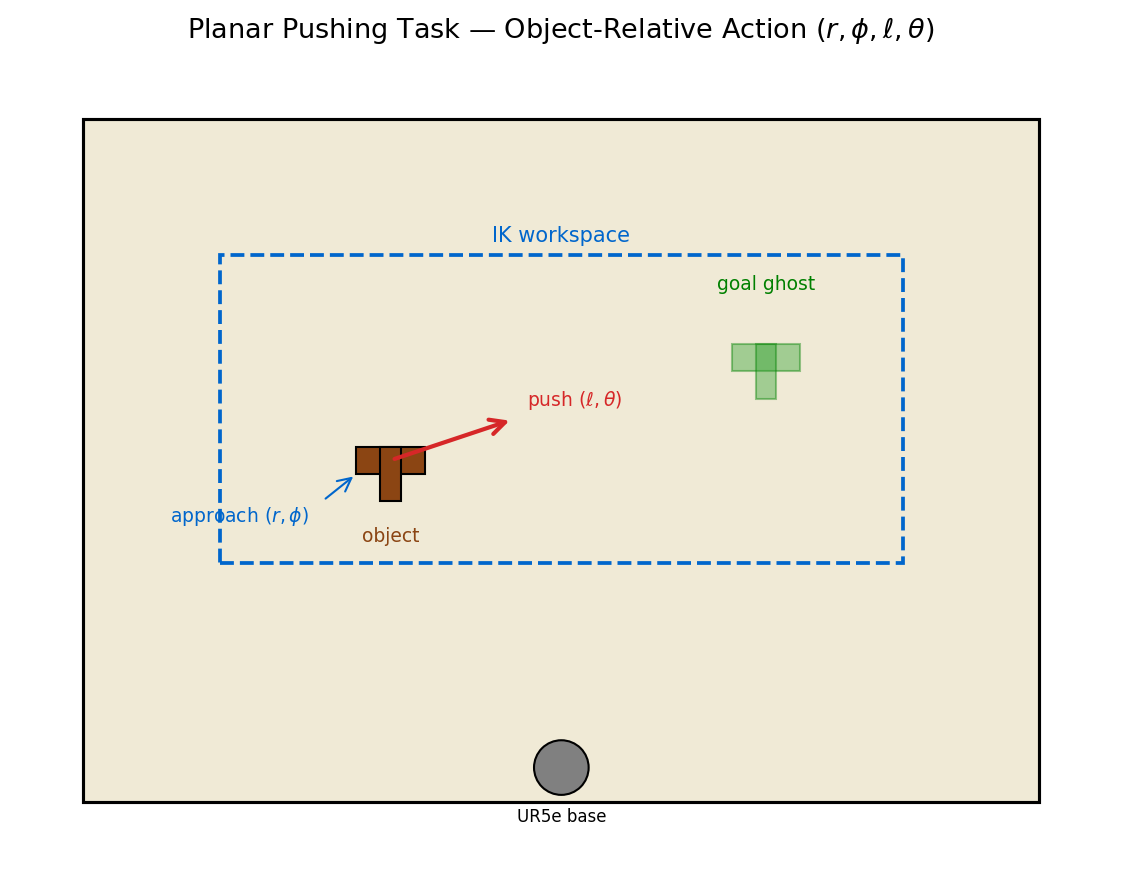
\includegraphics[width=0.55\textwidth]{diagram_task_schematic.png}
    \caption{The planar-pushing task. A UR5e arm pushes a T-block (blue) across a
    tabletop toward a goal pose (orange). Goals are defined in $\mathrm{SE}(2)$
    and combine a target position and a target orientation.}
    \label{fig:task_schematic}
\end{figure}

The principal advantage of Isaac Lab for this study is GPU-batched parallelism.
Many copies of the environment are stepped at the same time on a single device,
which produces the large sample batches on-policy learning requires. The
single-agent and curriculum models are trained with 528 parallel environments,
which yields a batch of roughly 7{,}920 push transitions per Proximal Policy
Optimization (PPO) update. A hardware upper bound of one RTX Pro 6000 GPU
(96\,GB of memory) sets the compute budget for every model, so all methods are
compared on equal terms. Inverse Kinematics (IK) for the arm is solved with
cuRobo 0.7.5, a GPU-accelerated batched IK solver.

\subsection{The Planar-Pushing Markov Decision Process}
\label{sec:mdp}

The task is modelled as an episodic Markov Decision Process (MDP) with a
macro-action, so that a single decision corresponds to one complete push rather
than to a low-level joint command.

\paragraph{State.}
The state is a 28-dimensional vector composed of four groups. These are the
end-effector pose (6 values), the object pose and velocity (14 values), the goal
pose (6 values), and the two scalar position and orientation errors between object
and goal. As explained in Section~\ref{sec:pomdp}, the current observation does
not report the underlying contact state. The problem is therefore formally
partially observable, and every policy is recurrent.

\paragraph{Action.}
The policy does not command joint torques. It selects an \emph{object-relative
push primitive} described by four parameters: a radial approach offset $r$, an
approach angle $\phi$ in the object frame, a push length $\ell$, and a push
direction $\theta$ in the world frame. Each parameter is discretised into 21 bins,
so the action is a four-dimensional MultiCategorical variable with $21^4 =
194{,}481$ discrete values. Parameterising the approach relative to the object,
rather than in absolute table coordinates, guarantees contact wherever the object
lies, which raises the contact rate to roughly 95\,\%. Once decoded, the primitive
runs as a five-phase trajectory, approach, descend, push, retract, and return,
spanning 72 physics substeps. Each waypoint is mapped to joint targets by the
cuRobo IK solver.

\paragraph{Transition.}
The object moves according to the quasi-static pushing mechanics of
Section~\ref{sec:pushing}. The limit-surface normality condition of
Equation~\ref{eq:normality} couples translation and rotation: almost every push
changes both the position and the orientation of the block. This coupling is a
property of the environment, not a modelling choice. It is the reason the task
cannot be decomposed into independent position and orientation sub-problems.

\paragraph{Reward.}
The reward is the subject of Sections~\ref{sec:frac_reward} to \ref{sec:se2}. It
is the single component that differs across the models compared in this thesis,
which is what makes the comparison a controlled one.

\paragraph{Success criterion.}
A push episode is counted as successful when the object is within
$0.05\,\text{m}$ of the goal position \emph{and} within $0.2\,\text{rad}$ of the
goal orientation. This combined gate is applied identically in training and
evaluation. The two conditions must hold at the same time, and the physics couples
the two axes. The combined gate is therefore the central difficulty of the task,
and the quantity every model is ultimately measured against.

\subsection{Why the Improvement Reward Fails}
\label{sec:frac_reward}

An initial baseline used a hand-tuned reward based on fractional improvement. It
rewards each push in proportion to the fraction of the remaining error it removes.
Let $d_{\text{prev}}$ and $d_{\text{now}}$ be the position error before and after
a push, and $y_{\text{prev}}$, $y_{\text{now}}$ the orientation error. The reward
is then
\begin{equation}
    R = \alpha\,\frac{d_{\text{prev}} - d_{\text{now}}}{d_{\text{prev}}}
        - \beta_{\text{pos}}\, d_{\text{now}}
        - \beta_{\text{rot}}\, y_{\text{now}},
    \qquad \alpha = 3.0,\; \beta_{\text{pos}} = 0.5,\; \beta_{\text{rot}} = 0.25.
    \label{eq:fractional}
\end{equation}

This reward performs poorly for two related reasons. Both concern the gradient it
supplies to PPO, not the optimal policy it defines. Consider a representative push
that moves the object $1\,\text{cm}$ closer to a goal $30\,\text{cm}$ away. The
improvement term contributes $3.0 \times 0.01/0.30 \approx 0.10$. The two penalty
terms contribute $-0.5 \times 0.29 \approx -0.145$ and $-0.25 \times 0.5 =
-0.125$, for a net reward of about $-0.17$. A push that makes genuine progress
therefore receives negative reward, because the standing penalty on the remaining
distance dominates the small improvement. This is the first problem: the reward is
negative for most useful pushes, so the policy gradient points away from
goal-directed behaviour.

The second problem is near-zero variance. Across a rollout, roughly 99\,\% of
pushes produce a reward in the narrow interval $[-0.5, +0.1]$, and the sparse
completion bonuses fire on about 1\,\% of pushes. At 528 environments and 15
pushes per rollout, only about 79 bonus events occur per iteration, too few to
overcome the noise in the dense term. The Generalized Advantage Estimation (GAE)
advantage is then dominated by noise, and the gradient is uninformative. The
failure is therefore one of gradient quality and reward variance, not of a
mis-specified optimum. The reward defines a reasonable objective but supplies a
poor learning signal.

\subsection{Potential-Based Reward Shaping for Pushing}
\label{sec:pbrs_design}

The remedy is to replace the improvement reward with a potential-based reward.
The per-push signal is then dense, correctly signed, and bounded, while the
optimal policy is provably unchanged (Section~\ref{sec:pbrs}). The design uses two
bounded exponential potentials, one for position and one for orientation:
\begin{align}
    \Phi_{\text{pos}}(s) &= w_{\text{pos}}\, \exp\!\left(-k_p\, d^2\right), \label{eq:phi_pos}\\
    \Phi_{\text{rot}}(s) &= w_{\text{rot}}\, \exp\!\left(-k_r\, c(s)\right),
    \qquad c(s) = \frac{1 - \cos(\theta^{*} - \theta)}{2}, \label{eq:phi_rot}
\end{align}
where $d$ is the planar position error and $c(s)$ is a cosine orientation
distance. The cosine form is smooth and free of the discontinuity a modular angle
difference would introduce at $\pm\pi$; $\theta^{*}$ and $\theta$ are the goal and
object yaw. The parameters are $k_p = 30$, $k_r = 5$, and $w_{\text{pos}} =
w_{\text{rot}} = 10$. The dense reward on a transition is the difference of the
summed potential,
\begin{equation}
    F(s, s') = \big[\Phi_{\text{pos}}(s') - \Phi_{\text{pos}}(s)\big]
             + \big[\Phi_{\text{rot}}(s') - \Phi_{\text{rot}}(s)\big],
    \label{eq:pbrs_dense}
\end{equation}
which is Equation~\ref{eq:pbrs} with $\gamma_{\text{shaping}} = 1$. The
undiscounted setting is admissible because the task is episodic and every episode
terminates, as established for episodic MDPs by \cite{Grzes2017RewardShaping}. Two
sparse bonuses are layered on the dense term. A completion bonus of $+5$ is given
when the position gate is satisfied, and a further $+2$ when the combined gate is
satisfied. A penalty of $-5$ is applied if the block tips over. These bonuses are
not themselves potential-based, but they fire only at terminal or near-terminal
events, where they do not create the reward-collecting cycles that
Section~\ref{sec:pbrs} identifies as the danger of non-potential shaping.

On the same representative push, the potential-based reward inverts the sign of
the baseline. For a $1\,\text{cm}$ improvement from $30\,\text{cm}$, the position
potential difference is $10 \times [\exp(-30 \times 0.29^2) - \exp(-30 \times
0.30^2)] \approx +0.13$. Every push toward the goal now receives positive reward,
and every push away from it negative reward. Because the potential is bounded in
$[0, w]$, the reward magnitude cannot be inflated by a physics contact spike.
Figure~\ref{fig:pbrs_signal} contrasts the per-push reward of the two schemes over
a representative episode, and shows the potential landscape and the gradient
comparison.

\begin{figure}[H]
    \centering
    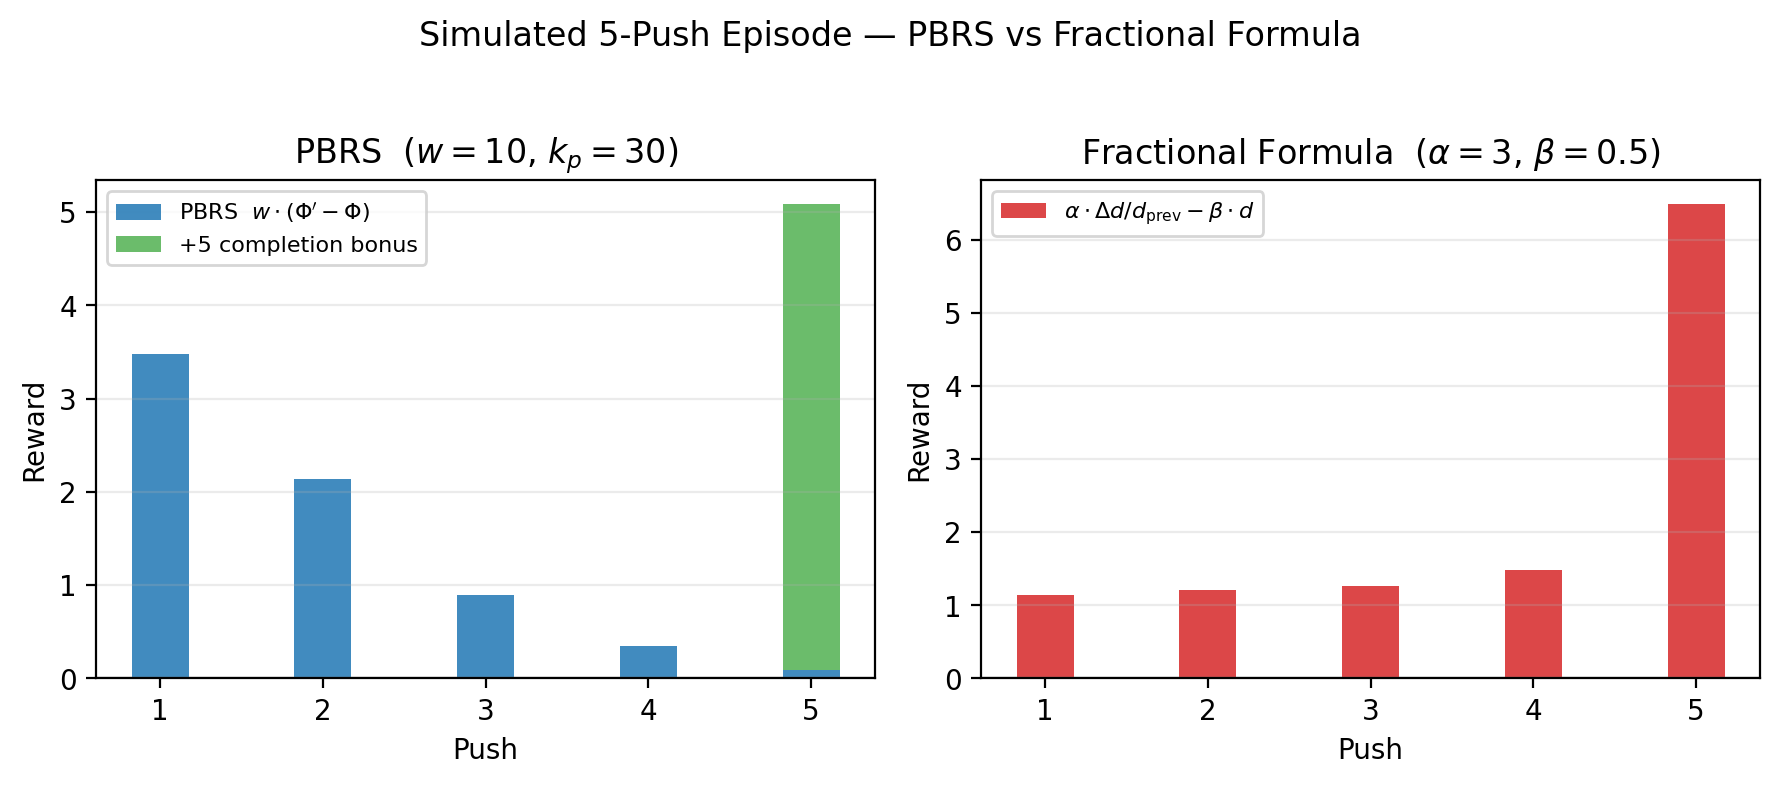
\includegraphics[width=0.48\textwidth]{a3_episode_simulation.png}\hfill
    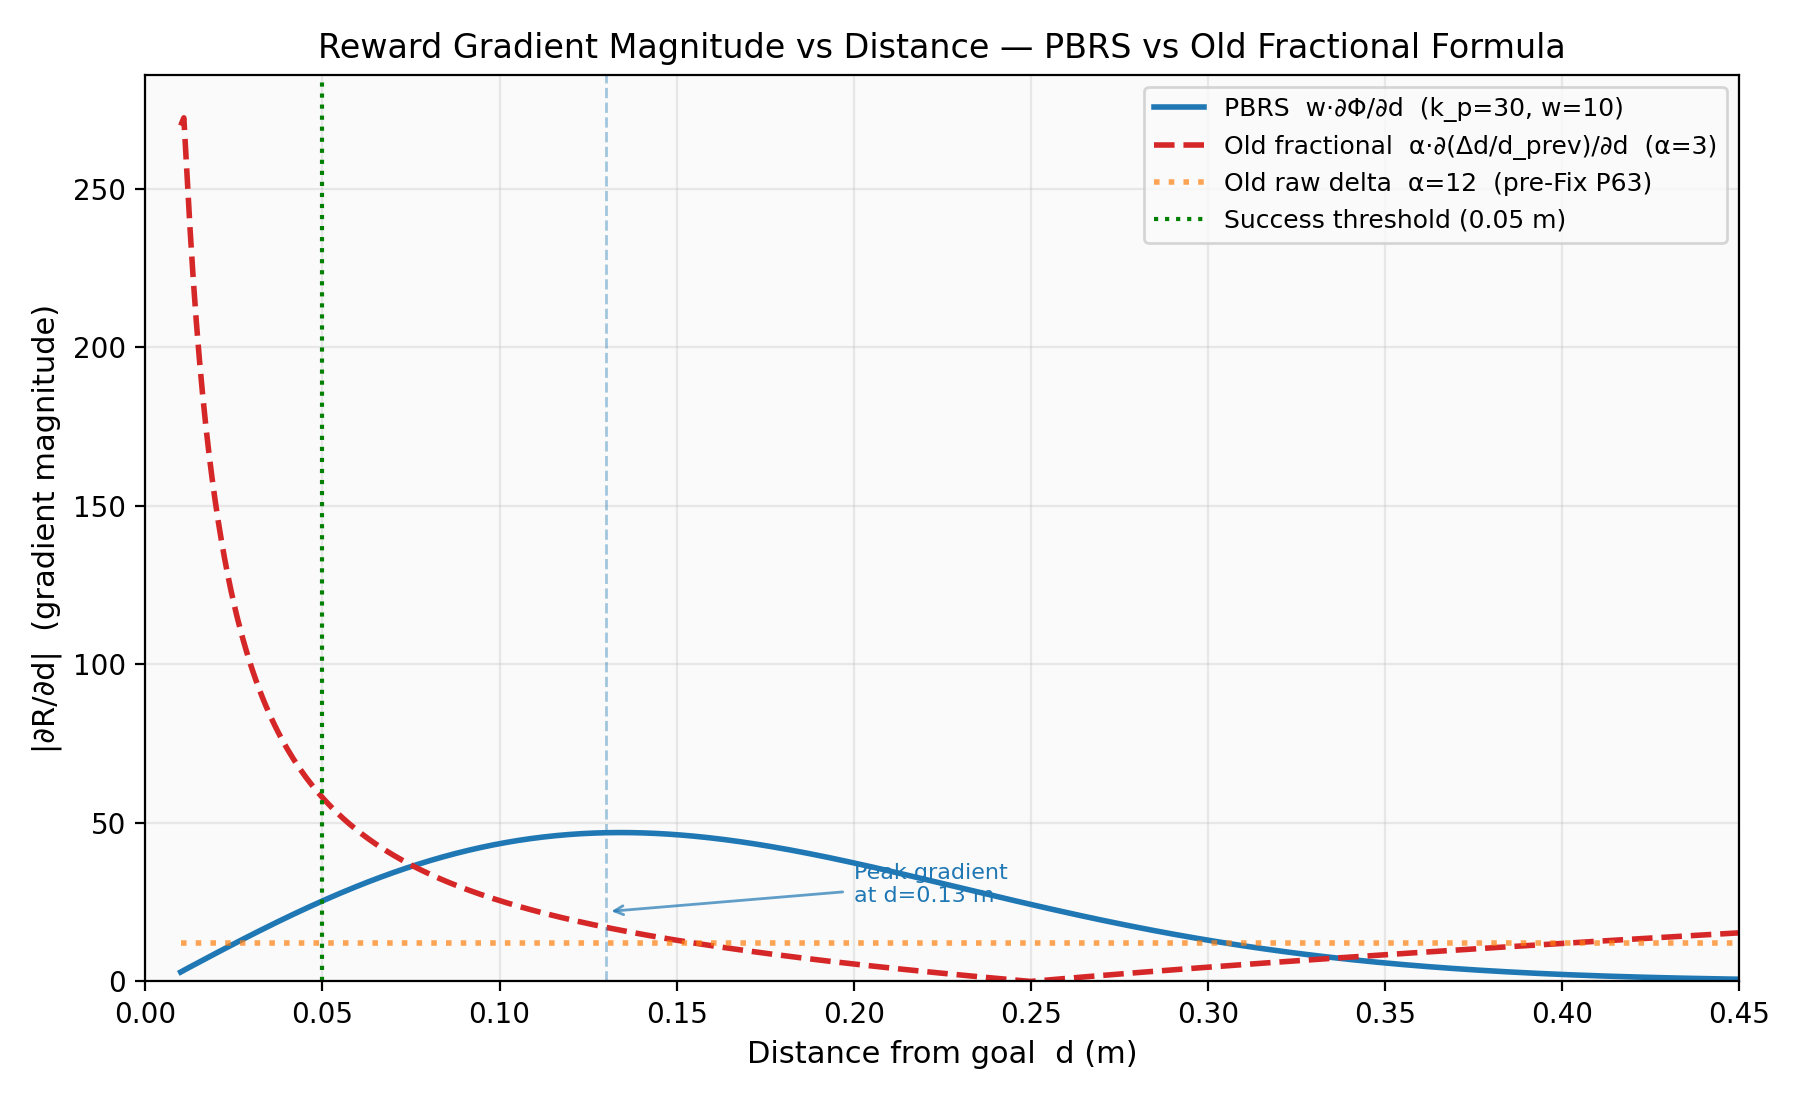
\includegraphics[width=0.48\textwidth]{a2_gradient_comparison.png}
    \caption{Left: per-push reward over a representative five-push episode for the
    improvement reward and the potential-based reward. The improvement reward is
    negative or near-zero for most pushes; the potential-based reward is
    correctly signed on every push. Right: the gradient supplied by the two
    schemes as a function of distance to the goal.}
    \label{fig:pbrs_signal}
\end{figure}

The reward is implemented as a potential-based reward function. Four properties
make it suitable for a contact-rich task, and all follow from its form. It is
Markovian, since it depends only on the current and successor state. It is
bounded. It produces zero net reward over any cycle that returns to the same
state, which removes the incentive for reward-collecting loops. And it produces
zero reward while the object is stationary, so it imposes no penalty for
deliberation.

\subsection{The SE(2) Unified Distance}
\label{sec:se2}

The two-potential reward treats position and orientation as separate terms whose
gradients can point in different directions. For the self-play models
(Section~\ref{sec:models}) the reward instead uses a single $\mathrm{SE}(2)$
distance, so one potential governs the whole pose. Following the Lie-group
formulation of Section~\ref{sec:pushing}, the pose error is summarised by the
scalar
\begin{equation}
    d_{\text{pose}} = \sqrt{\Delta x^2 + \Delta y^2 + L^2\, \Delta\theta^2},
    \label{eq:dpose_methods}
\end{equation}
where $\Delta x$, $\Delta y$ are the position error components and $\Delta\theta$
the orientation error. Here $L$ is a characteristic length that converts an
angular error into an equivalent linear displacement. For the T-block $L =
0.07\,\text{m}$, the block's radius of gyration; it is a physical property of the
object, not a tuning parameter. The corresponding single potential and its dense
reward are
\begin{equation}
    \Phi_{\text{pose}}(s) = w\, \exp\!\left(-k\, d_{\text{pose}}^2\right),
    \qquad F(s,s') = \Phi_{\text{pose}}(s') - \Phi_{\text{pose}}(s),
    \label{eq:phi_dpose}
\end{equation}
with $k = 30$ and $w = 10$. The success threshold for this metric is
$d_{\text{pose}} < 0.055\,\text{m}$ for the T-block. The single potential removes
the competing-gradient problem of the two-potential form. A push that reduces
$d_{\text{pose}}$ is rewarded whether the reduction comes from position or
orientation, so the reward is aligned with the coupled physics of the task. Both
the two-potential and the unified formulations share the same reward
implementation.

\subsection{The Five Models}
\label{sec:models}

All five models share the same backbone: a single PPO agent with an LSTM of
hidden size 256 followed by a multilayer perceptron, and a MultiCategorical head
over the four-dimensional, 21-bin push primitive. They differ only in the reward
and the training dynamics, which is what makes the comparison controlled. The
five models are summarised in Table~\ref{tab:models}.

\begin{table}[H]
    \centering
    \small
    \begin{tabularx}{\textwidth}{l l X}
        \hline
        \textbf{Model} & \textbf{Training dynamics} & \textbf{Reward} \\
        \hline
        PPO-Baseline & single agent & improvement reward (Equation~\ref{eq:fractional}) \\
        PPO-PBRS & single agent & two-potential PBRS (position, orientation) \\
        PPO-Curriculum & single agent, staged & two-potential PBRS with forced position-then-orientation staging \\
        ASP-dPose & asymmetric self-play & $\mathrm{SE}(2)$ PBRS for Bob, outcome-based Alice reward \\
        TASP-dPose & asymmetric self-play & $\mathrm{SE}(2)$ PBRS for Bob, time-based Alice reward \\
        \hline
    \end{tabularx}
    \caption{The five models. Every model uses the same PPO+LSTM backbone and the
    same object-relative push primitive; only the reward and the training
    dynamics change.}
    \label{tab:models}
\end{table}

\paragraph{PPO-Baseline.}
A single PPO agent trained with the improvement reward of
Equation~\ref{eq:fractional}. It serves as the reference point for the reward
comparison of Section~\ref{sec:frac_reward} and is trained at 2{,}048 parallel
environments, a larger batch than the other models use.

\paragraph{PPO-PBRS.}
A single PPO agent trained with the two-potential reward of
Equations~\ref{eq:phi_pos} to \ref{eq:pbrs_dense}. This is the simplest model that
uses the potential-based reward, with no curriculum and no second agent, and it
is trained at 528 environments.

\paragraph{PPO-Curriculum.}
PPO-PBRS with a forced three-phase curriculum that stages the two objectives.
Phase 1 trains position only, with the orientation weight set to zero. Phase 2
begins when the episodic position-only success rate reaches 0.5 over a
20-iteration window; the orientation weight is then increased from 0 to 10 over
200 iterations. Phase 3 is the full two-objective reward. The trigger gates on the
episodic position-only success rate, rather than on a per-push error mean. This is
the corrected version of a trigger that in an earlier implementation never
activated; the earlier failure and its correction are documented in Appendix~H.

\paragraph{ASP-dPose.}
An asymmetric self-play model that uses the $\mathrm{SE}(2)$ reward of
Equation~\ref{eq:phi_dpose} for the goal-solving agent, Bob. The loop is shown in
Figure~\ref{fig:asp_loop}. The goal-setting agent, Alice, performs five pushes to
propose a goal. The goal is accepted only if it passes a validity check: the block
has moved sufficiently, remains on the table, and lies inside the workspace. Bob
then attempts the goal from a clean reset over up to ten pushes. Alice's reward is
\emph{outcome-based}, following \cite{OpenAI2021AsymmetricSF}: she receives a
reward when Bob fails, a shaping bonus for a valid goal, and a penalty for an
out-of-bounds goal. Bob additionally uses a GoalEncoder, a small multilayer
perceptron that maps the six-dimensional goal pose into an eight-dimensional
latent, in the difference variant of \cite{Sukhbaatar2018GoalEmbeddings}. Bob is
trained with Alice Behavioral Cloning at $\beta = 0.5$.

\paragraph{TASP-dPose.}
Identical to ASP-dPose except that Alice's reward is \emph{time-based}, following
\cite{Sukhbaatar2018IntrinsicMotivation}: $R_A = \gamma_{sp}\max(0, t_B - t_A)$.
This rewards Alice for proposing goals that take Bob more pushes to solve than
Alice took to set, subject to a penalty on Alice's own effort. It is the
self-regulating reward of Equation~\ref{eq:sukh_alice}. The two self-play models
therefore differ only in Alice's reward, which isolates the effect of the goal
proposal mechanism.

\begin{figure}[H]
    \centering
    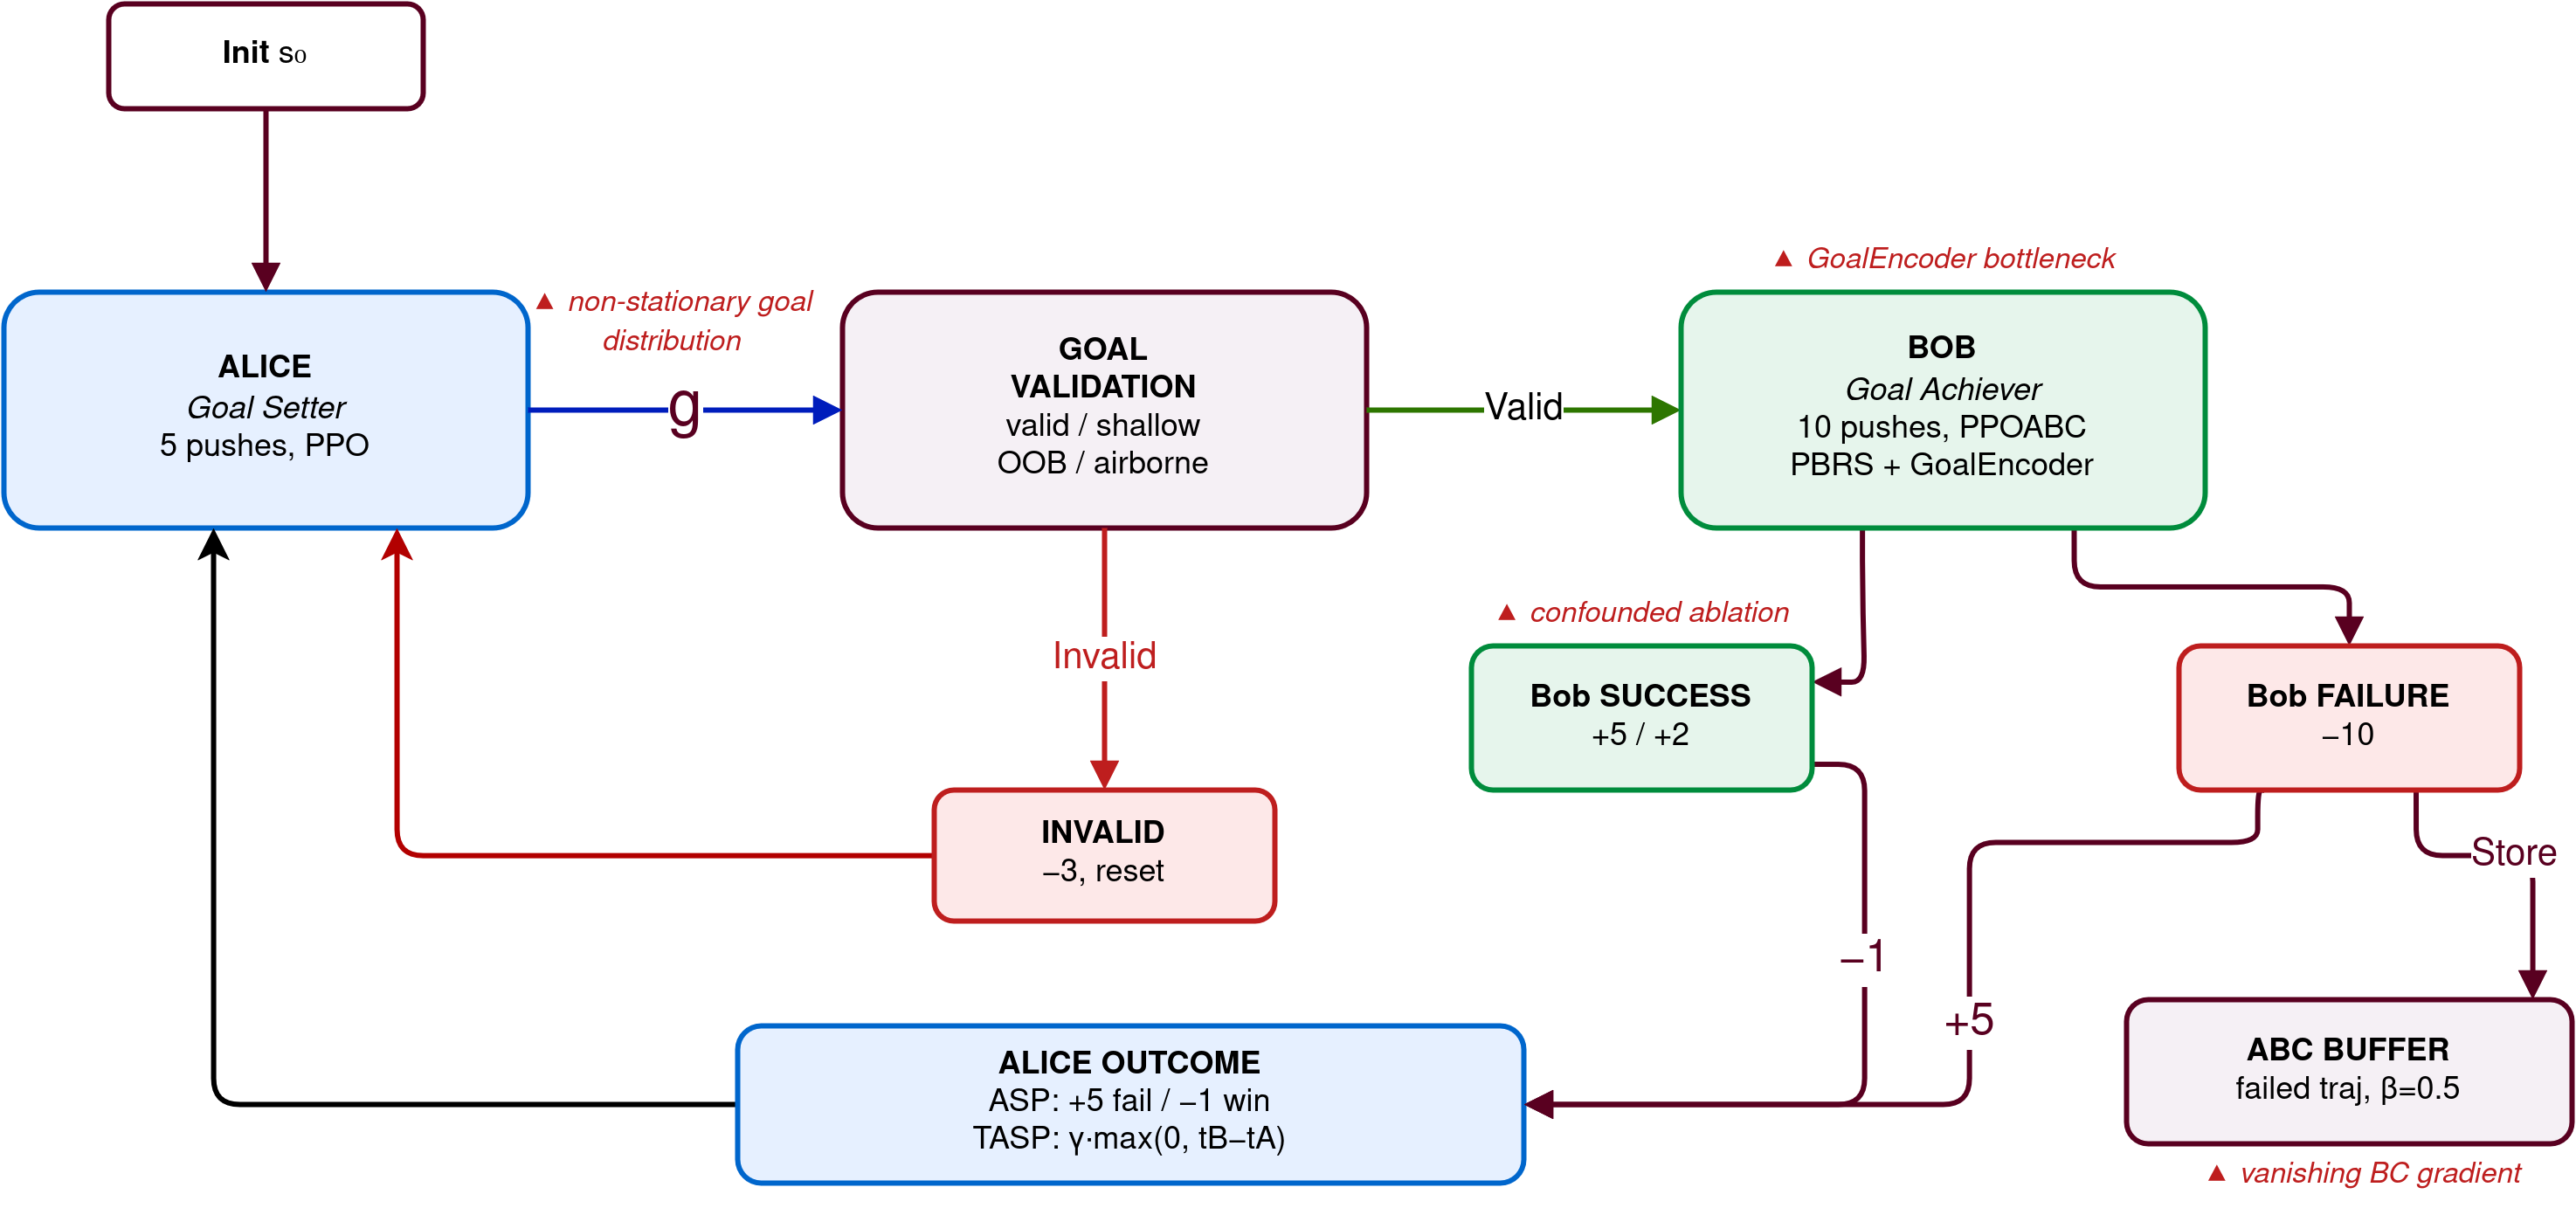
\includegraphics[width=0.9\textwidth,height=0.5\textheight,keepaspectratio]{asp_loop_diagram.png}
    \caption{The asymmetric self-play loop. Alice proposes a goal by acting for a
    fixed number of pushes; the goal is validated; Bob then attempts it from a
    clean reset. Alice's reward differs between ASP-dPose (outcome-based) and
    TASP-dPose (time-based); Bob's $\mathrm{SE}(2)$ potential-based reward is the
    same in both.}
    \label{fig:asp_loop}
\end{figure}

\subsection{Why PBRS Assists Self-Play but Does Not Solve It}
\label{sec:pbrs_asp}

Potential-based shaping improves self-play but does not make it competitive with
single-agent training, and the reason is visible in the structure of the GAE
advantage. The advantage estimate is a discounted sum of one-step temporal
differences, each of which decomposes into a reward term and a value-bootstrap
term:
\begin{equation}
    \hat{A}_t = \sum_{l \geq 0} (\gamma\lambda)^l
    \underbrace{\big[\Phi(s_{t+l+1}) - \Phi(s_{t+l})\big]}_{\text{potential term, correctly signed}}
    \;+\; \sum_{l \geq 0} (\gamma\lambda)^l
    \underbrace{\big[\gamma V(s_{t+l+1}) - V(s_{t+l})\big]}_{\text{value term, biased when } V \text{ is stale}}.
    \label{eq:gae_decomp}
\end{equation}
The potential term is correctly signed on every push, regardless of the accuracy
of the value function, because the potential increases whenever the object moves
toward the goal. The value term, by contrast, depends on the accuracy of $V$. In
single-agent training the goal distribution is stationary, so $V$ is accurate and
both terms agree. Under self-play, Alice changes the goal distribution at every
iteration, so $V$ is perpetually estimated on a distribution that no longer holds,
and the value term is biased. The potential term supplies a floor of correct
learning signal, which lifts self-play above the level it reaches under the sparse
or improvement reward. It cannot, however, remove the bias contributed by the
stale value term. The consequence, quantified in Chapter~\ref{sec:results}, is
that
potential-based shaping raises self-play from near-zero to a modest success rate
without approaching the single-agent result.

This account is a hypothesis about the learning dynamics, not a result. Both of
its claims, the elevated value error under a shifting goal distribution and the
suppression of the imitation signal, are measured directly through the training
instrumentation described in Section~\ref{sec:instrumentation}, and the
measurements are reported in Chapter~\ref{sec:results} rather than asserted here.

\subsection{Experimental Campaign Overview}
\label{sec:campaign}

The five models of Section~\ref{sec:models} are the objects of study. A single
training run of each, at one batch size and one seed, cannot support the
statistical and causal claims this thesis makes. The evaluation is therefore
organised as a campaign of budget-matched training runs, summarised in
Table~\ref{tab:campaign}. Its per-phase configurations and job counts are given in
Chapter~\ref{sec:experiments}. This section states the two principles that make
the campaign a controlled study, together with the validation protocol and
training instrumentation that every run shares. The numerical outcomes appear in
Chapter~\ref{sec:results}.

The first principle is \textbf{multiple seeds with reported confidence intervals}.
Single-seed reinforcement-learning results are known to be unreliable, because the
variance between random seeds can exceed the difference between methods
\cite{Henderson2018DeepRLMatters, Agarwal2021StatisticalPrecipice}. Every headline
comparison in this thesis is therefore repeated across several seeds. Each is
reported as a mean with a 95\,\% confidence interval, so a claimed difference
between two models is distinguished from seed noise.

The second principle is \textbf{budget matching}. The aim is to compare batch
sizes without confounding them with the amount of experience. The total number of
pushes seen over training is therefore held constant while the number of parallel
environments is varied. The iteration count is set inversely proportional to the
number of environments, so each configuration consumes the same total experience
of about 23.8 million pushes. The temporal window of the recurrent policy is fixed
at 15 pushes per rollout; only the number of parallel environments, and therefore
the per-update batch size, changes. This isolates the per-update batch size, the
quantity that drives the value-function bias of Section~\ref{sec:pbrs_asp}, from
the total experience.

\begin{table}[H]
    \centering
    \small
    \begin{tabularx}{\textwidth}{l l X}
        \hline
        \textbf{Phase} & \textbf{Question} & \textbf{Design} \\
        \hline
        Scale sweep & Does the self-play deficit close as the batch grows? &
        the two self-play models across four environment counts \\
        Environment frontier & How few environments does each single-agent reward need? &
        potential-based single agent and the improvement-reward baseline across four environment counts, three seeds \\
        Seed intervals & Are the model differences larger than seed noise? &
        single agent, curriculum, and both self-play models at the anchor budget, five seeds \\
        Self-play ablations & Which component of the self-play package matters? &
        the self-play model with the goal encoder, behavioural cloning, or the historical pool removed one at a time, three seeds \\
        Positive control & Does behavioural cloning help on an easy symmetric task? &
        self-play on the rotationally symmetric disc with behavioural cloning enabled, three seeds \\
        Reward sensitivity & Is the potential-based reward robust to its parameters? &
        the single agent over a grid of the position sharpness $k_p$ and the potential weight $w$ \\
        Cross-environment & Does the ordering hold in a second simulator? &
        single agent, curriculum, and self-play in the two-dimensional pushing simulator across two batch sizes \\
        \hline
    \end{tabularx}
    \caption{The experimental campaign. Each phase answers one question flagged in
    review; the per-phase training configurations, environment counts, seeds, and
    job counts are tabulated in Chapter~\ref{sec:experiments}.}
    \label{tab:campaign}
\end{table}

\subsection{Validation Protocol}
\label{sec:val_protocol_methods}

Every trained policy is evaluated on the same held-out suite of 30 T-block
scenes, illustrated in Figure~\ref{fig:val_layout_methods}. The suite is divided
into three groups of ten. The first ten are rotation-dominant scenes with large
orientation changes. The next ten are position-only scenes whose goal orientation
equals the start orientation. The last ten are combined scenes that require both a
position and an orientation change. Within each group the difficulty ranges from
easy to hard, graded by the start-to-goal distance and the required rotation. The
held-out scenes are fixed in advance and never seen during training, so
performance on them measures generalisation rather than memorisation.

\begin{figure}[H]
    \centering
    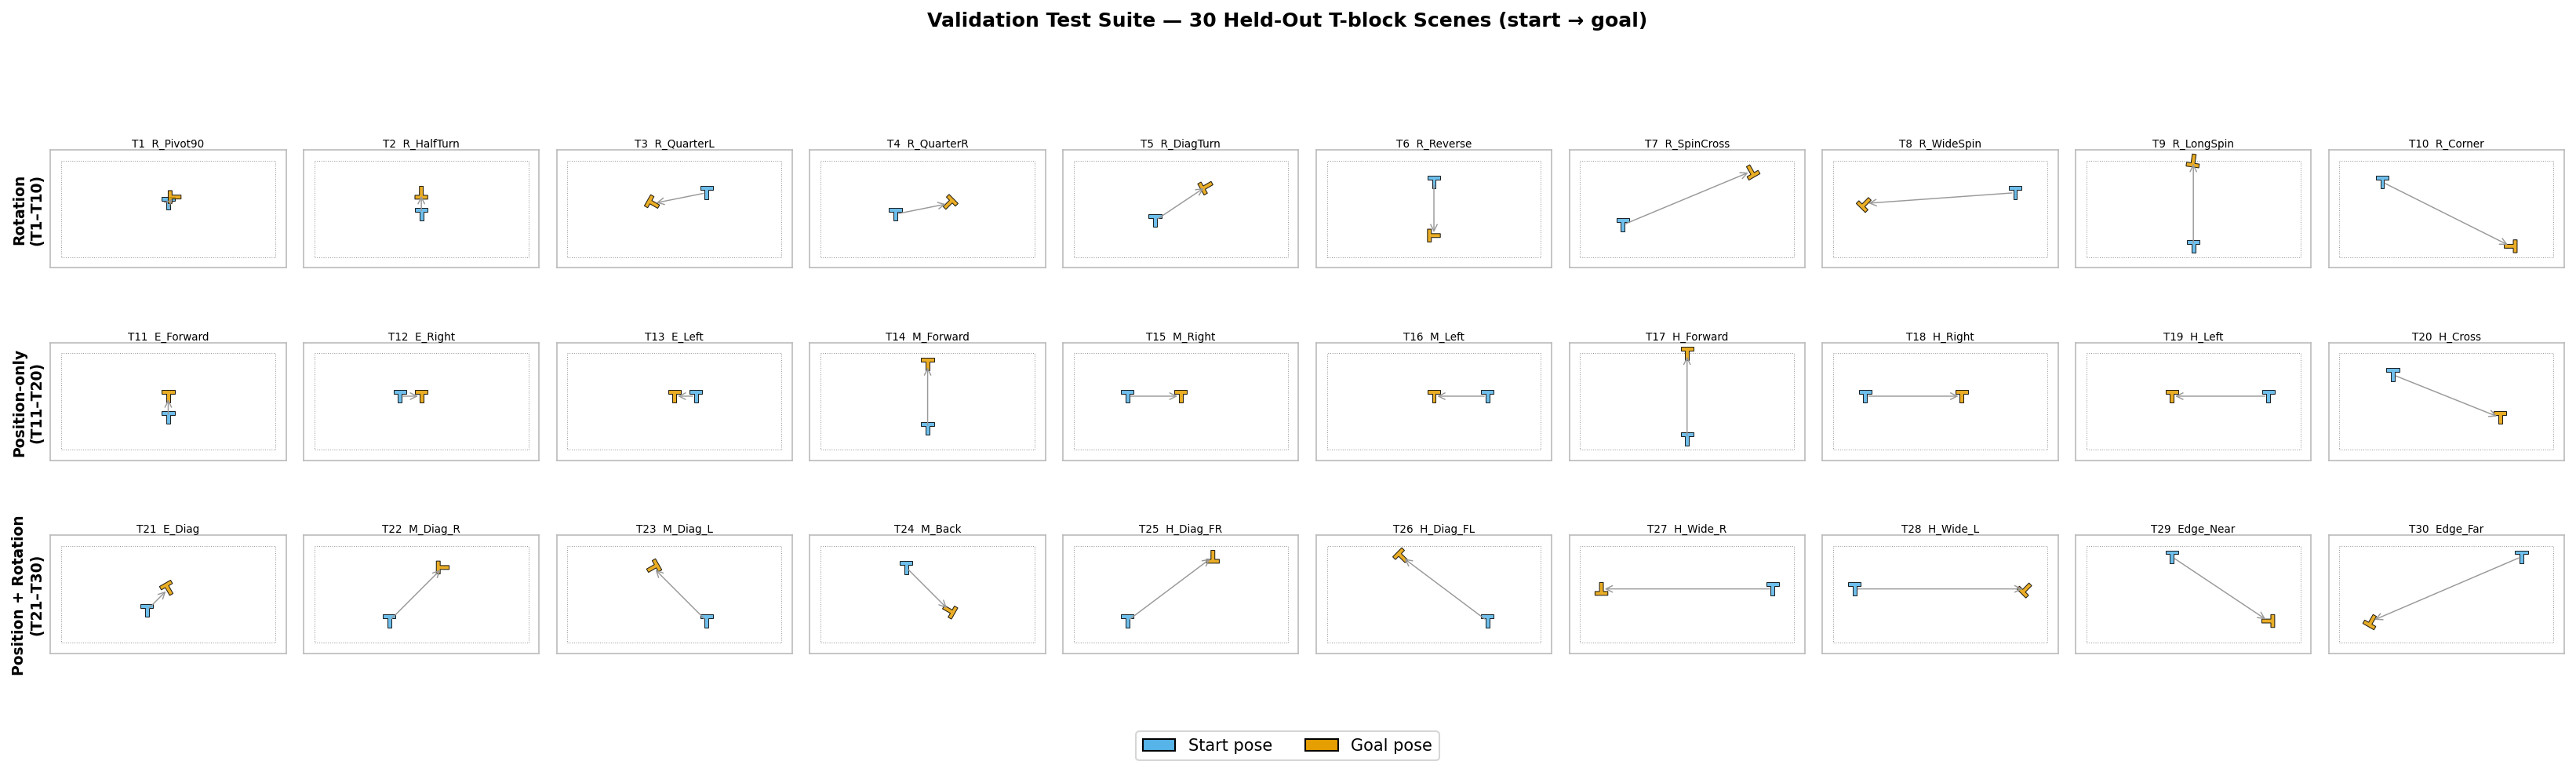
\includegraphics[width=\textwidth,height=0.42\textheight,keepaspectratio]{val_test_layout.png}
    \caption{The 30-scene held-out validation suite. Each panel shows the block
    start pose and the goal pose for one scene. The suite is identical for every
    model and every seed.}
    \label{fig:val_layout_methods}
\end{figure}

Each scene is attempted 20 times, and within each attempt the policy is allowed
up to 30 pushes. Two success measures are reported and kept distinct throughout
the thesis. The \textbf{scene success rate} counts a scene as solved if at least
one of its 20 attempts satisfies the combined gate of Section~\ref{sec:mdp}. This
is the headline measure, and follows the convention common in manipulation
evaluation, where a task counts as achievable if the policy can achieve it at all.
The \textbf{trial success rate} is the fraction of individual attempts that satisfy
the gate, and is always the lower of the two. Reporting both prevents the
best-of-20 protocol from overstating performance, and the gap between them is
stated wherever the headline number appears.

Three protocol decisions make the numbers comparable across models. Each corrects
a subtle way the comparison could otherwise be invalidated. First, the checkpoint
selected for validation is the one that maximised the \emph{combined}
position-and-orientation success rate during training, not the looser
single-distance threshold used internally by the self-play reward. Selecting on a
different criterion than the one reported would flatter the self-play models.
Second, the self-play policies trained on the rotationally symmetric disc are
validated on disc scenes, whose goal orientation is unconstrained, not on the
T-block scenes they never trained on. Validating an agent on a task it never
trained for would void its result. Third, checkpoints that lack a combined-gate
best model, and are validated only from their latest checkpoint, are recorded
separately and excluded from the confidence-interval aggregation. A
partially-trained run therefore cannot contaminate a headline mean. The per-seed
results are aggregated into a mean with a 95\,\% confidence interval per model,
batch size, and iteration count.

\subsection{Training Instrumentation for the Self-Play Mechanism}
\label{sec:instrumentation}

The account in Section~\ref{sec:pbrs_asp} of why potential-based shaping only
partially assists self-play rests on two claims. The first is that the
value-function term of the advantage estimate is biased under the shifting goal
distribution. The second is that the behavioural-cloning signal is suppressed when
the goal-proposing agent's demonstrated actions lie far from the goal-solving
agent's policy. Rather than leave these as arguments, the training runs are
instrumented so that both are measured directly, and the measurements are reported
in Chapter~\ref{sec:results}.

For the value-function claim, the mean absolute difference between the value
estimates and the empirical returns is logged at every policy update. This is done
for the single-agent, self-play, and time-based self-play models alike. Under the
budget-matched scale sweep, this quantity can be plotted against the number of
parallel environments. The mechanism of Section~\ref{sec:pbrs_asp} makes two
predictions: the value error is larger under self-play than under single-agent
training at the same batch size, and it falls as the batch grows. A value error
that declines toward the single-agent level with scale would support a
budget-limitation account. One that remains elevated would indicate a structural
deficit independent of budget.

For the behavioural-cloning claim, the imitation term is instrumented in three
ways: the share of demonstrated actions whose probability ratio falls outside the
clipping interval, the mean ratio, and the mean probability the goal-solving agent
assigns to the goal-proposing agent's demonstrated actions. The clipping mechanism
inherited from the imitation loss of \cite{OpenAI2021AsymmetricSF} zeroes the
gradient for any demonstrated action whose ratio leaves the trust interval. A large
clipped fraction is therefore the direct signature of a suppressed imitation
signal. Measuring this fraction converts the clip-saturation account into a
reported quantity. A positive control on the rotationally symmetric disc, where
behavioural cloning is enabled and the task is easy, tests whether the mechanism
can help at all in this setting. If imitation assists anywhere it should assist
there, so its failure on the coupled T-block task cannot then be dismissed as a
broken implementation.


% !TEX root = ../main.tex
\section{Experimental Setup}
\label{sec:experiments}

This chapter describes how the nine models of Chapter~\ref{section:methods} are
trained and evaluated. It specifies the tools and hardware, the training
configuration and the experiment set, and the held-out validation protocol. It
then describes the cross-environment comparison against a second simulator, an
off-policy baseline based on Soft Actor-Critic, and the metrics reported in the
results.

\subsection{Tools and Infrastructure}
\label{sec:tools}

Training and Isaac-Lab evaluation run on a single RTX Pro 6000 GPU with 96\,GB of
memory. The software stack is Isaac Sim 5.1.0, Isaac Lab 2.3.0, cuRobo 0.7.5 for
batched Inverse Kinematics (IK), and PyTorch 2.7.0. A second environment, the
two-dimensional \texttt{gym-pusht} simulator, is used for the cross-environment
comparison of Section~\ref{sec:cross_env}. It runs on 32 CPU cores and uses
neither IK nor three-dimensional contact physics. The off-policy baseline of
Section~\ref{sec:sac_baseline} uses Stable-Baselines3 2.7.0. Running the same
models in two simulators of different fidelity separates conclusions that hold
across environments from artefacts of a single implementation.

\subsection{Training Configuration and the Experiment Set}
\label{sec:train_config}

At the 528-environment anchor, every model is trained for approximately 3{,}000
iterations. This corresponds to about 1.6 days of wall-clock time per model on the
RTX Pro 6000. At 15 pushes per rollout it yields a batch of roughly 7{,}920 push
transitions per PPO update. For the reward-efficiency comparison, the
improvement-reward baseline and the potential-based agent are trained across the
same environment counts, from 256 to 2{,}048, so the two rewards are measured at
matched parallelism rather than at a single batch. The two self-play subjects are
additionally trained at 256 and 2{,}048 environments, which tests whether the
single-GPU compute budget is the cause of their result. The PPO hyperparameters are
a learning rate of $3\times10^{-4}$, a clipping range of 0.2, a discount factor of
0.998, a GAE parameter of 0.95, and an entropy coefficient of 0.005. The self-play
models additionally use Alice Behavioral Cloning at $\beta = 0.5$.

Two points about the training history are stated for reproducibility. First, all
reported checkpoints post-date a sequence of corrections to the reward and the
environment. The reported numbers are therefore produced on the corrected code,
and earlier runs are excluded. Second, the improvement-reward baseline and the
potential-based agent are compared across a shared range of environment counts, so
that any difference between the two rewards cannot be attributed to unequal
parallelism. The budgets are tabulated in Appendix~K.

Every Isaac Lab run in the experiment set is budget-matched. The total experience
is held at about 23.8 million pushes, and the iteration count is set inversely
proportional to the number of parallel environments, so a change in the number of
environments changes the per-update batch size alone. This design has one confound that is
stated wherever a scale result appears: a larger batch also means fewer gradient
updates over training, so batch size and update count move together and cannot be
fully separated. Table~\ref{tab:phases} lists the phases, the models each one
trains, the environment counts, the matched iteration counts, and the seeds.

\begin{table}[H]
    \centering
    \small
    \begin{tabularx}{\textwidth}{l X c c c c}
        \hline
        \textbf{Phase} & \textbf{Models} & \textbf{Envs} & \textbf{Iterations} &
        \textbf{Seeds} & \textbf{Runs} \\
        \hline
        Anchor and efficiency & PPO-Baseline, PPO-PBRS & 256--2{,}048 &
        773--6{,}188 & 3 & 24 \\
        Seed intervals & Baseline, PBRS, Curriculum, ASP-dPose, TASP-dPose & 528 &
        3{,}000 & 5 & 25 \\
        Coupling isolation & ASP-disc, TASP-disc & 528 & 3{,}000 & 5 & 10 \\
        Self-play scale & ASP-dPose, TASP-dPose & 256, 2{,}048 & 6{,}188; 773 & 3 &
        12 \\
        Component ablations & ASP-dPose, TASP-dPose & 528 & 3{,}000 & 3 & 12 \\
        Imitation positive control & ASP-disc & 528 & 3{,}000 & 3 & 6 \\
        Reward structure & Bob-penalty & 528 & 3{,}000 & 5 & 5 \\
        Cross-environment & single agent, curriculum, self-play & 64, 256 &
        3{,}000 & 1 & 10 \\
        \hline
    \end{tabularx}
    \caption{The phases of the experiment set. Environments and iterations trade
    off to hold the total experience at about 23.8 million pushes for the Isaac Lab
    runs; the cross-environment runs instead use a fixed 3{,}000 iterations and a
    single seed, and vary the per-update batch through the environment count and
    the push length. The experiment set comprises 94 training runs in Isaac Lab and
    10 in the second simulator.}
    \label{tab:phases}
\end{table}

\subsection{Validation Protocol}
\label{sec:val_protocol}

Every model is evaluated on the same held-out suite of 30 T-block scenes,
illustrated in Figure~\ref{fig:val_layout}. The suite is divided into three groups
of ten. The first ten are rotation-dominant scenes with large orientation
changes. The next ten are position-only scenes whose goal orientation equals the
start orientation. The last ten are combined scenes that require both a position
and an orientation change. Within each group the difficulty ranges from easy to
hard, graded by the start-to-goal distance and the magnitude of the required
rotation.

\begin{figure}[H]
    \centering
    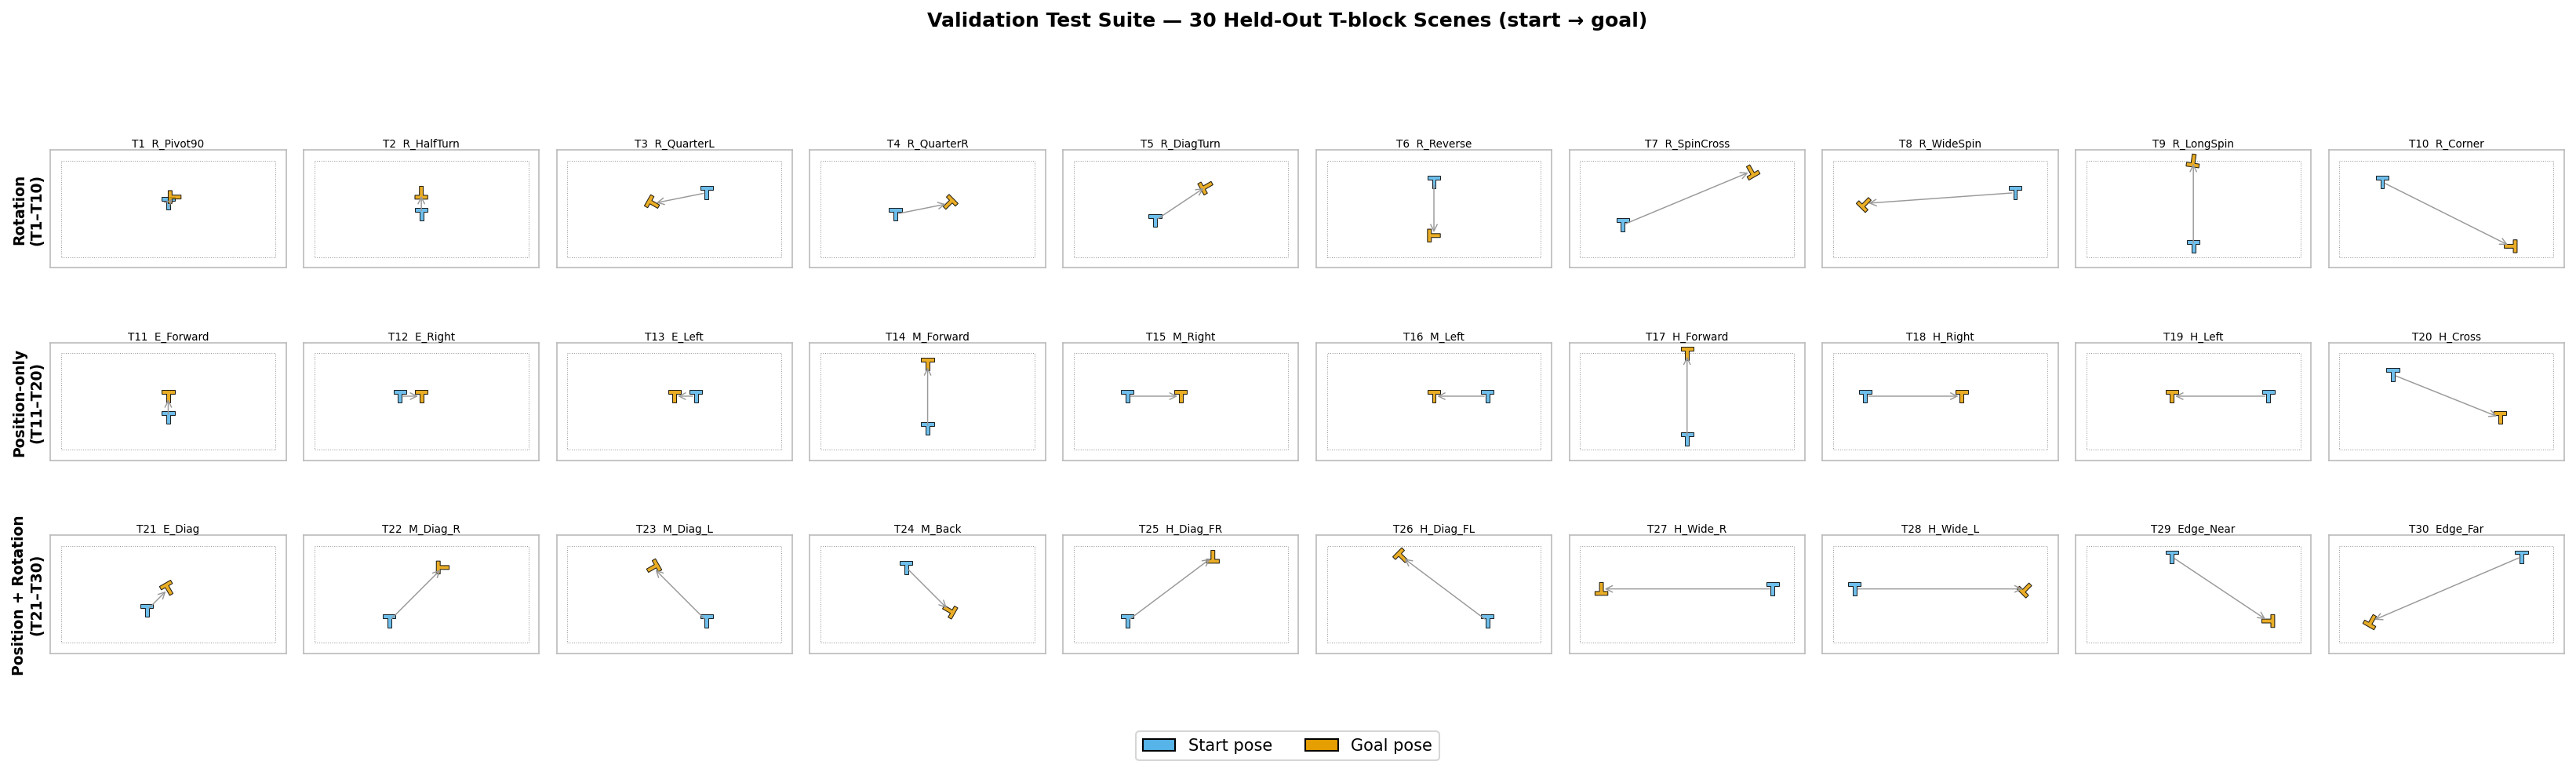
\includegraphics[width=\textwidth,height=0.42\textheight,keepaspectratio]{val_test_layout.png}
    \caption{The 30-scene held-out validation suite. Each panel shows the block
    start pose and the goal pose for one scene. The suite is identical for every
    model.}
    \label{fig:val_layout}
\end{figure}

Each scene is attempted 20 times, and within each attempt the policy is allowed up
to 30 pushes. Both the single-agent and the self-play validators sample actions
from the policy, rather than taking the most probable action, so every model is
scored under one protocol. Two success measures are reported and kept distinct
throughout. The \emph{scene success rate} counts a scene as solved if at least one
of its 20 attempts satisfies the combined gate of Section~\ref{sec:mdp}. This is
the headline number, and follows the convention common in manipulation evaluation.
The \emph{trial success rate} is the fraction of individual attempts that satisfy
the gate, and is always lower than the scene success rate. Reporting both prevents
the best-of-20 protocol from overstating performance, and the gap between them is
stated wherever the headline number appears; the final values are \TBD until the
seed runs are collated. Each model is evaluated across its trained seeds, and the
results are aggregated into a mean with a 95\,\% confidence interval per model,
batch size, and iteration count.

\subsection{Cross-Environment Protocol}
\label{sec:cross_env}

To test whether the ordering of the models is a property of the methods rather
than of Isaac Lab, the single-agent, curriculum, and self-play models are
retrained and evaluated in \texttt{gym-pusht} under the same 30-scene gate. The
two environments differ mainly in the size of the PPO batch. Isaac Lab produces
about 7{,}920 transitions per update at the 528-environment anchor, while
\texttt{gym-pusht} produces between about 960 and 11{,}520, depending on the
environment count and the push length. The gym runs use a fixed 3{,}000 iterations
and sweep the per-update batch through these two settings, so the comparison tests
whether the ordering of the methods survives a second, lower-fidelity simulator,
rather than matching the total experience between the two environments.
Figure~\ref{fig:isaac_vs_gym} summarises the throughput and batch size of the two
environments.

\begin{figure}[H]
    \centering
    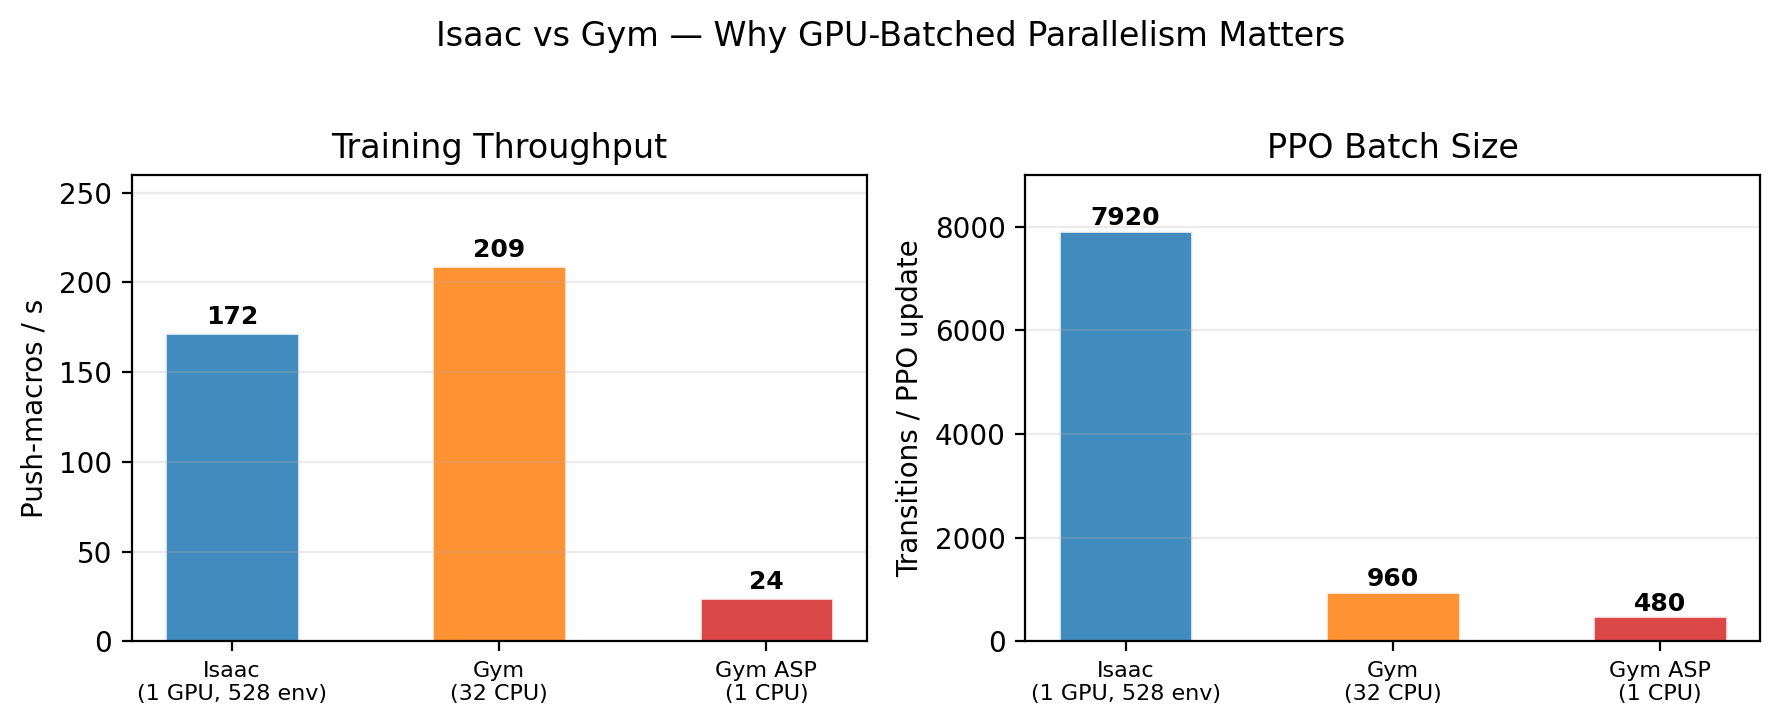
\includegraphics[width=0.7\textwidth,height=0.4\textheight,keepaspectratio]{isaac_vs_gym.png}
    \caption{Throughput and PPO batch size for Isaac Lab and \texttt{gym-pusht}.
    Raw throughput is comparable; the per-update batch differs by roughly a factor
    of eight, which is the variable the cross-environment comparison isolates.}
    \label{fig:isaac_vs_gym}
\end{figure}

\subsection{Off-Policy Baseline: SAC with Hindsight Experience Replay}
\label{sec:sac_baseline}

The principal models are all on-policy. To provide an external point of
calibration from a different algorithm family, an off-policy baseline is built
from Soft Actor-Critic (SAC) \cite{Haarnoja2018SoftAO} combined with Hindsight
Experience Replay (HER) \cite{Andrychowicz2017}. SAC is a natural counterpart to
PPO for this problem. It is sample-efficient through experience replay, and its
maximum-entropy objective (Equation~\ref{eq:sac}) supports exploration under
sparse reward. HER addresses the sparse goal-conditioned setting directly: it
relabels the object pose actually reached in a failed attempt as if it had been
the goal, so every attempt yields usable transitions.

The baseline runs on a direct control environment through Stable-Baselines3, and
reuses the shared push primitive and the cuRobo IK pipeline of
Section~\ref{sec:mdp}. Two adaptations are required. First, SAC is a
continuous-action algorithm, so the four push parameters become a continuous
action in $[-1, 1]^4$ and are decoded to the same object-relative primitive,
rather than the MultiCategorical variable used by the PPO models. Second, the
goal-conditioned observation is expressed in the dictionary form the replay buffer
expects, with separate observation, achieved-goal, and desired-goal entries. The
baseline is trained and evaluated under the same 30-scene protocol as the
principal models, so its success rate is directly comparable. Its role is
calibration rather than competition. It indicates whether an off-policy,
replay-based method reaches performance similar to the on-policy potential-based
model, and its status against the compute budget is reported with the results.

\subsection{Metrics}
\label{sec:metrics}

The results report the following quantities, each with its sample size and
protocol stated at the point of use. The primary metric is the scene success rate
over the 30-scene suite, with the trial success rate reported alongside it. The
breakdown by scene type, position-only against combined, is reported because it
localises where each model fails. Mean position error and mean orientation error
are reported as continuous measures of near-misses. For the self-play models the
training logs also provide the per-axis success rates: the fraction of pushes that
satisfy the position gate alone and the orientation gate alone. These are compared
against the combined-gate rate to diagnose whether the two skills are learned but
not combined. Average push count per attempt is reported as a measure of
efficiency. Three further quantities are logged during self-play training and
reported in the results. The first is the mean absolute value error, which
measures the bias of the value function under the shifting goal distribution. The
second is the share of demonstrated actions the imitation term clips away, a direct
measure of how strongly the imitation signal is suppressed. The third is the
Alice-replay rate: the fraction of proposed goals that the goal-proposing agent's
own action sequence reaches when replayed from the goal-solving agent's start
state. All reported numbers trace to the validation records summarised in the
results.


% !TEX root = ../main.tex
\section{Results}
\label{sec:results}

This chapter reports the generalisation of every model to the held-out 30-scene
suite, organised by research question. Section~\ref{sec:rq_baseline} establishes
that the task is solvable. Section~\ref{sec:rq1} addresses whether asymmetric
self-play succeeds under the single-GPU budget (RQ1). Section~\ref{sec:rq2}
isolates the setup dimension that separates success from failure (RQ2).
Section~\ref{sec:rq3} identifies the underlying mechanism (RQ3).
Section~\ref{sec:cross_env_results} reports the second-simulator result.

Three success measures are reported and kept distinct throughout, and all are
defined in Section~\ref{sec:metrics}. The
\emph{held-out scene success rate} is computed on the fixed 30-scene suite that no
model saw during training, and is the measure of generalisation this thesis reports
as its headline. The \emph{within-distribution scene success rate} is computed on
goals drawn from the model's own training distribution, and its gap against the
held-out rate is the mechanism of Section~\ref{sec:rq3}. The \emph{training-time
success rate} is an auxiliary per-push rate computed on the goals the models
trained on. Unless stated otherwise, headline models report 5 seeds at 528
environments; ablations and scale sweeps report 3 seeds; confidence intervals are
95\,\% across seeds. The held-out numbers in this chapter follow the evaluation
protocol defined in Section~\ref{sec:val_protocol}, and every comparison reported
here is already decisive under that protocol.
Table~\ref{tab:main_results} collects the principal numbers.

\begin{table}[H]
    \centering
    \small
    \begin{tabular}{l c c c c}
        \hline
        \textbf{Model} & \textbf{Scene SR} & \textbf{Trial SR} & \textbf{Pos-only} & \textbf{Seeds} \\
        \hline
        PBRS (potential-based)   & \textbf{79.3\,\% $\pm$ 3.5\,\%} & 70.2\,\% & 100\,\% & 5 \\
        Curriculum               & \textbf{80.0\,\% $\pm$ 4.1\,\%} & 70.2\,\% & 100\,\% & 5 \\
        ASP-disc (position-only) & 7.3\,\% $\pm$ 1.8\,\%  & 5.8\,\% & --- & 5 \\
        TASP-disc                & 6.7\,\% $\pm$ 0.0\,\%  & 4.9\,\% & --- & 5 \\
        ASP-dPose (outcome)      & 0.0\,\%                & 0.0\,\% & 0\,\%  & 5 \\
        TASP-dPose (time-based)  & 0.0\,\%                & 0.0\,\% & 0\,\%  & 4 \\
        Bob-penalty              & 0.0\,\%                & 0.0\,\% & 0\,\%  & 4 \\
        \hline
    \end{tabular}
    \caption{Held-out generalisation of the headline models at 528 environments.
    Scene SR counts a scene solved if any of its attempts passes the combined gate;
    trial SR is the per-attempt rate. Pos-only is the scene SR on the ten
    position-only scenes. Values are seed means with 95\,\% confidence intervals
    across seeds, under the evaluation protocol of Section~\ref{sec:val_protocol}.}
    \label{tab:main_results}
\end{table}

\subsection{Baseline}
\label{sec:rq_baseline}

The single-agent models establish that the task is solvable, which is the
precondition for interpreting any self-play result as a property of the method
rather than the task. PBRS reaches a held-out scene success rate of
79.3\,\% ($\pm$ 3.5 percentage points, 5 seeds) at 528 environments, and the
curriculum model reaches 80.0\,\% ($\pm$ 4.1\,pp, 5 seeds). On the ten
position-only scenes both reach 100\,\%; on the twenty scenes that also require
an orientation change they reach 69\,\% and 70\,\%. The single-agent models
therefore fail only on rotation-requiring scenes, and never because of position.
Their trial success rate of 70.2\,\% shows that the policy is reliable as well as
capable: a scene is solved in the majority of attempts, not in a single lucky one.
The per-scene errors of Figure~\ref{fig:per_scene_errors} show where the
remaining failures concentrate: position error stays below tolerance on every
scene, and the unsolved scenes are those whose orientation error exceeds
the 0.2\,rad threshold.

The single-agent models show no generalisation gap. Their training goals are
sampled uniformly over the workspace, so the within-distribution evaluation of
Section~\ref{sec:metrics} draws goals from the same distribution as the held-out
suite, and the two success rates coincide. The 79.3\,\% held-out result is
therefore also the single-agent's within-distribution competence. This
distinguishes the single-agent models from the self-play models of
Section~\ref{sec:rq3}, whose within-distribution success collapses on the
held-out suite.

\begin{figure}[H]
    \centering
    \includegraphics[width=\textwidth,height=0.5\textheight,keepaspectratio]{per_scene_errors_3models.png}
    \caption{Per-scene generalisation errors, seed means across 5 seeds
    ($\pm$ 1 standard deviation). Top row: position error; bottom row:
    orientation error. Columns: PBRS, Curriculum, and ASP-dPose. Green bars mark
    scenes solved in the majority of seeds; the dashed line marks the combined-gate
    threshold. The single-agent models leave only rotation-dominant scenes
    unsolved, while ASP-dPose solves none.}
    \label{fig:per_scene_errors}
\end{figure}

\subsection{Research Question 1: ASP performance under the single-GPU budget}
\label{sec:rq1}

The self-play models do not generalise to the held-out suite at all. ASP-dPose
and TASP-dPose each solve zero of the 30 scenes, in every seed (5 and 4 seeds
respectively). The Bob-penalty model is likewise at zero. This is not a
marginal underperformance against the 79\,\% of the single-agent model; it is a
complete failure to transfer.

The two Alice reward formulations are indistinguishable at this level. The
outcome-based reward of \cite{OpenAI2021AsymmetricSF} and the time-based reward
of \cite{Sukhbaatar2018IntrinsicMotivation} both produce zero held-out successes,
so the reward-formulation dimension cannot be resolved on the T-block: both variants
fail entirely. The same holds for the symmetric Bob-penalty variant. The failure
is one of transfer, not of learning. On goals the goal-proposing agent itself
produces, the self-play policy solves 61.4\,\% of disc scenes and 11.7\,\% of
T-block scenes (5 seeds each, Section~\ref{sec:rq3}), and none of that
competence reaches the held-out suite. The
comparisons that can be made at this level are between the within-distribution
behaviour of Section~\ref{sec:rq3} and the held-out result, where a consistent
picture emerges.

The disc models, whose goal constrains position alone, are marginally above
zero. ASP-disc solves 7.3\,\% of its 30 disc scenes ($\pm$ 1.8\,pp, 5 seeds) and
TASP-disc 6.7\,\% ($\pm$ 0.0\,pp, 5 seeds). The couple of scenes each disc model
solves are the easiest of the suite. This places the disc contrast of
Section~\ref{sec:rq2_coupling} in its proper light: self-play fails on both
objects, and fails completely on the coupled-goal T-block.

\begin{figure}[H]
    \centering
    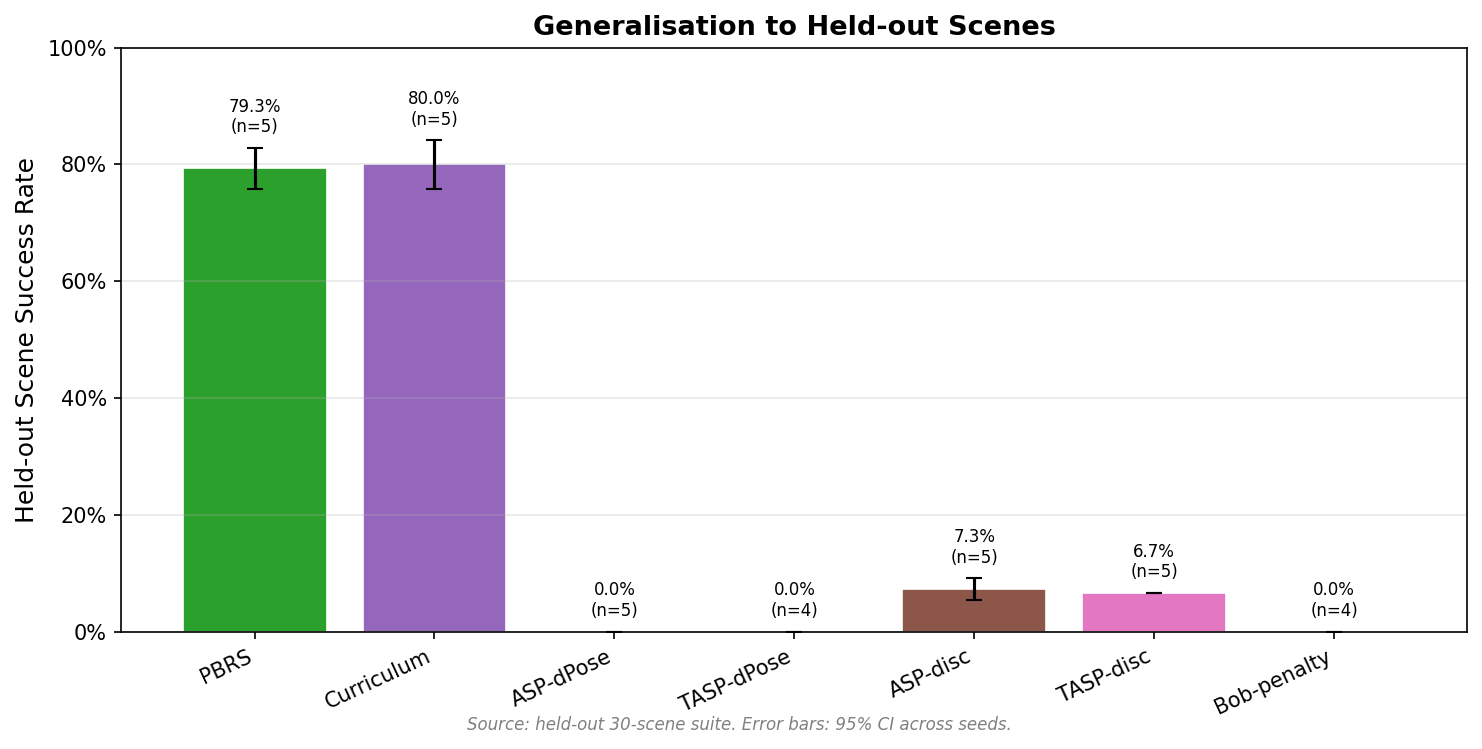
\includegraphics[width=\textwidth,height=0.45\textheight,keepaspectratio]{val_multi_combined.png}
    \caption{Held-out scene success rates for the headline models at 528
    environments. The single-agent models solve roughly four scenes in five; the
    disc self-play models solve fewer than one in ten; the T-block self-play
    models solve none.}
    \label{fig:val_multi}
\end{figure}

\subsection{Research Question 2: Setup dimensions}
\label{sec:rq2}

This section reports the single-dimension isolations that decompose the self-play
result. Each isolates one factor that differs between the successful prior
settings and the present setup.

\subsubsection{Goal Coupling}
\label{sec:rq2_coupling}

The disc self-play models isolate the coupled goal as a single variable. On the
rotationally symmetric disc, whose goal constrains position alone, self-play
solves 7.3\,\% of held-out scenes. On the T-block, whose goal couples position
and orientation, the same mechanism solves 0.0\,\%. The pose, the push primitive,
the Bob reward, and the self-play loop are identical between the two variants;
only the object and the success criterion differ.

The within-distribution evaluation of Section~\ref{sec:rq3} measures the coupling
directly. On goals the goal-proposing agent itself generates, the disc model
solves 61.4\,\% of scenes ($\pm$ 2.1\,pp, 5 seeds) while the T-block model
solves 11.7\,\% ($\pm$ 1.5\,pp, 5 seeds). The coupled gate therefore reduces
within-distribution competence by roughly 50 percentage points before any
transfer is required. The held-out suite then collapses both rates, the disc to
7.3\,\% and the T-block to zero. The failure thus separates into two effects of
comparable size. The coupled gate accounts for the within-distribution drop from
61.4\,\% to 11.7\,\%; the generalisation collapse accounts for the drop from each
within-distribution rate to its held-out rate, roughly 54 percentage points on
the disc. Neither effect alone explains the full result, and the second is the
subject of Section~\ref{sec:rq3}.

The single-agent models show the same gate effect in a solvable setting. On the
ten position-only scenes they reach 100\,\%; on the twenty scenes that also
demand an orientation change they reach 69--70\,\%. The coupled gate is hard even
for the model that solves the task, which is why it compounds self-play's
generalisation failure decisively.

\subsubsection{Reward Formulation}
\label{sec:rq2_reward}

The two Alice reward formulations produce identical held-out outcomes: zero
scenes solved for both ASP-dPose and TASP-dPose. The self-regulating property of
the time-based reward of \cite{Sukhbaatar2018IntrinsicMotivation} does not confer
a measurable advantage in this setup, and neither reward transfers. The
reward-formulation dimension is therefore not the factor that
separates the successful prior settings from this one: both formulations fail
equally here.

\subsubsection{Compute Scale}
\label{sec:rq2_scale}

The two self-play subjects were trained at 256, 528, and 2{,}048 parallel
environments with matched total experience, so that the per-update batch size
varies while the total pushes stay fixed. On the held-out suite ASP-dPose solves
0.0\,\% of scenes at 256 and 528 environments (3 and 5 seeds), and 1.1\,\%
($\pm$ 4.8\,pp, 3 seeds) at 2{,}048, where a single seed solves a single scene.
TASP-dPose solves 0.0\,\% at all three counts. An eightfold increase in the
parallel batch does not lift the self-play result above the noise floor. Compute
scale is therefore ruled out as the cause of the underperformance, in the
strongest sense available: the curve is not merely flat, it is flat at zero.

\subsubsection{Imitation Signal}
\label{sec:rq2_abc}

The imitation term introduced by \cite{OpenAI2021AsymmetricSF}, Alice
Behavioural Cloning at $\beta = 0.5$, is instrumented through the fraction of
demonstrated actions whose probability ratio falls outside the clipping interval.
For every ABC-enabled model this clip fraction is \textbf{0.000} at every
training iteration: the goal-proposing agent's exploratory pushes lie so far from
the goal-solving agent's policy that the clipping zeroes the gradient, and the
imitation signal never flows.

The ablation shows the signal's absence has no measurable effect because there
is nothing left to preserve. Removing ABC changes the held-out scene SR of ASP-dPose from
0.0\,\% to 0.0\,\% (3 seeds), and the same holds for TASP-dPose and for the disc
models (6.7\,\% with and without). The positive control on the disc, where the
task is easiest and the imitation term would be most likely to help, also shows
no effect. The practical consequence is that the imitation term contributes
nothing in this discrete macro-action domain; the clip-saturation measurement
explains why.

\subsubsection{Goal Representation}
\label{sec:rq2_encoder}

Removing the GoalEncoder from Bob and providing the full object-and-goal
observation directly to the policy encoder changes the held-out scene SR of
ASP-dPose from 0.0\,\% to 0.0\,\% (3 seeds). The eight-dimensional latent
compression is not the factor that limits self-play, consistent with the disc
isolation, where the same encoder is present and self-play retains its marginal
generalisation.

\subsection{Research Question 3: Mechanism}
\label{sec:rq3}

The mechanism of the self-play failure is the gap between the within-distribution
competence and the held-out performance.
Table~\ref{tab:rq3} and Figure~\ref{fig:train_heldout} place the two measures
side by side.

\begin{table}[H]
    \centering
    \small
    \begin{tabular}{l c c c}
        \hline
        \textbf{Model} & \textbf{Within-dist SR} & \textbf{Held-out SR} & \textbf{Seeds} \\
        \hline
        ASP-disc     & 61.4\,\% $\pm$ 2.1\,\%  & 7.3\,\%          & 5 \\
        ASP-dPose    & 11.7\,\% $\pm$ 1.5\,\%  & 0.0\,\%          & 5 \\
        \hline
    \end{tabular}
    \caption{Within-distribution against held-out scene success for the two
    self-play subjects. Within-distribution SR is the scene success rate on goals
    proposed by the frozen goal-proposing agent and accepted by the validity
    check, under the evaluation protocol of Section~\ref{sec:val_protocol};
    held-out SR is the 30-scene rate. Values are seed means with 95\,\%
    confidence intervals across the seeds listed. The single-agent models are
    omitted because their uniform training goal distribution coincides with the
    held-out suite, so their within-distribution and held-out rates are the same.}
    \label{tab:rq3}
\end{table}

The within-distribution evaluation separates the two effects that the headline
numbers confound. On goals the goal-proposing agent itself produces, the disc
model solves 61.4\,\% of scenes and the T-block model 11.7\,\%, across five seeds
each. The same models solve 7.3\,\% and 0.0\,\% of held-out scenes. The
single-agent models show no such separation: their uniform training goal
distribution coincides with the held-out suite, so their within-distribution and
held-out rates agree at roughly 79\,\%.

Two effects of comparable size are now measurable. The first is the coupled
gate. Within the proposer's own distribution, replacing the position-only disc
goal with the coupled T-block goal reduces scene success from 61.4\,\% to
11.7\,\%, a drop of roughly 50 percentage points. The second is the
generalisation collapse. The disc model loses a further 54 percentage points
between its within-distribution rate and the held-out suite, and the T-block
model falls from 11.7\,\% to zero. The coupled gate therefore bounds competence
on the proposer's own goals, while the narrow goal distribution prevents that
competence from transferring.

The per-axis training logs confirm that the coupled gate, not a missing skill,
limits the T-block. ASP-dPose satisfies the position gate on 41.0\,\% of its
training pushes and the rotation gate on 33.9\,\%, yet the combined gate is met
on only 11.7\,\% of within-distribution scenes. The two skills are present but
rarely co-satisfied. On the disc, where only position is demanded, the
within-distribution rate rises to 61.4\,\%, which confirms that the coupling is
what suppresses the T-block within-distribution. The residual transfer failure,
in which even the disc's competence does not reach the held-out suite, is a
property of the goal distribution itself. Alice proposes goals near her own final
pose, so the policy is trained on goals the held-out suite never presents, and
its competence is tied to those goals rather than to a transferable skill.

This answers RQ3. Self-play does not fail because a component of the method is
broken, and it does not fail from a single cause. Two effects compound: the
coupled multi-objective gate reduces the competence the policy acquires on its
own goals by roughly 50 percentage points, and the narrow goal distribution
prevents that competence from reaching the held-out suite. Both follow from the
same curriculum, and together they reduce the disc's 61.4\,\% to a held-out
7.3\,\% and the T-block's 11.7\,\% to zero.

\begin{figure}[H]
    \centering
    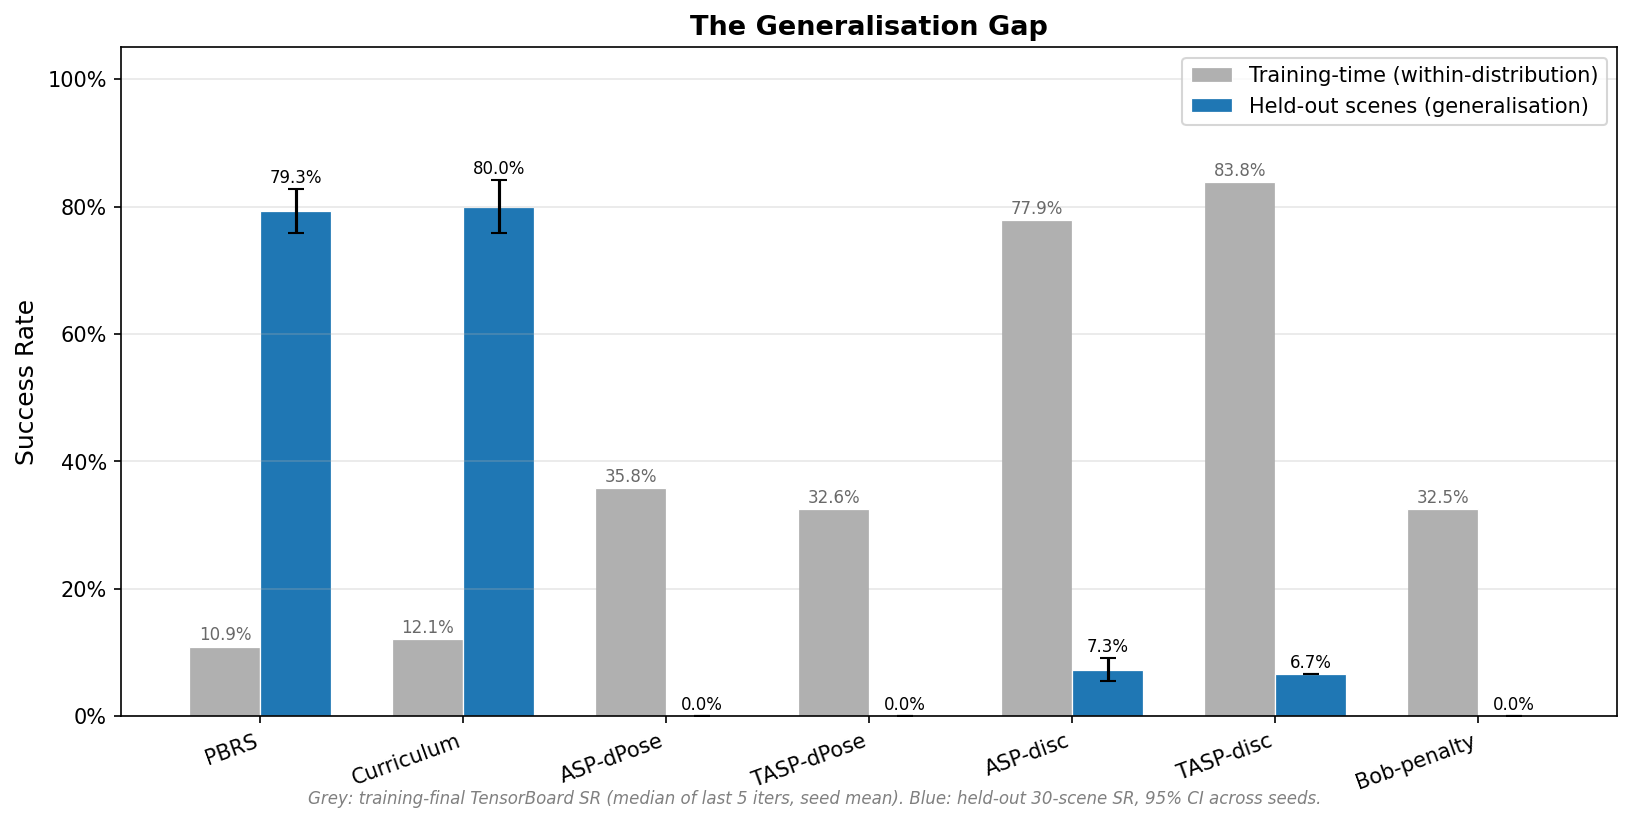
\includegraphics[width=\textwidth,height=0.42\textheight,keepaspectratio]{asp_diagnostic_2panel.png}
    \caption{The generalisation gap. Grey bars: within-distribution scene
    success rate (seed mean). Blue bars: held-out scene success rate with
    95\,\% confidence intervals. The single-agent models show no gap, because
    their training goal distribution coincides with the held-out suite; the
    self-play models collapse from their within-distribution rate to the held-out
    rate.}
    \label{fig:train_heldout}
\end{figure}

\subsection{Cross-Environment}
\label{sec:cross_env_results}

The second-simulator counterpart provides a single-seed qualitative check, and
each number below rests on that one seed. The numbers come from the primary
configuration of 64 environments and 15 pushes per rollout; the remaining
configurations of Section~\ref{sec:cross_env} are training-only. The
single-agent model solves 3.3\,\% of the 30 scenes, far below the 79.3\,\% of
the Isaac Lab model. The curriculum counterpart solves 9.0\,\%, and the
self-play counterpart solves 1.0\,\%. The lower absolute rates reflect the lower
fidelity of the second simulator and its single seed, not a contradiction of the
Isaac Lab result. What transfers is the ordering. The self-play model remains
the weakest of the three in both simulators. The curriculum model matches or
exceeds the plain single-agent model, consistent with the curriculum comparison
of Chapter~\ref{sec:conclusion}.

\subsection{Qualitative Behaviour}
\label{sec:qualitative}

Figure~\ref{fig:keyframes} shows keyframes of the single-agent PBRS policy
solving three held-out scenes. The policy approaches the block along the
object-relative offset, pushes along the decoded direction, and repeats until the
combined gate is met. Its failures, on the rotation-dominant scenes, show
position under control and orientation outside the 0.2\,rad tolerance, which
matches the per-type breakdown of Table~\ref{tab:main_results}.

\begin{figure}[H]
    \centering
    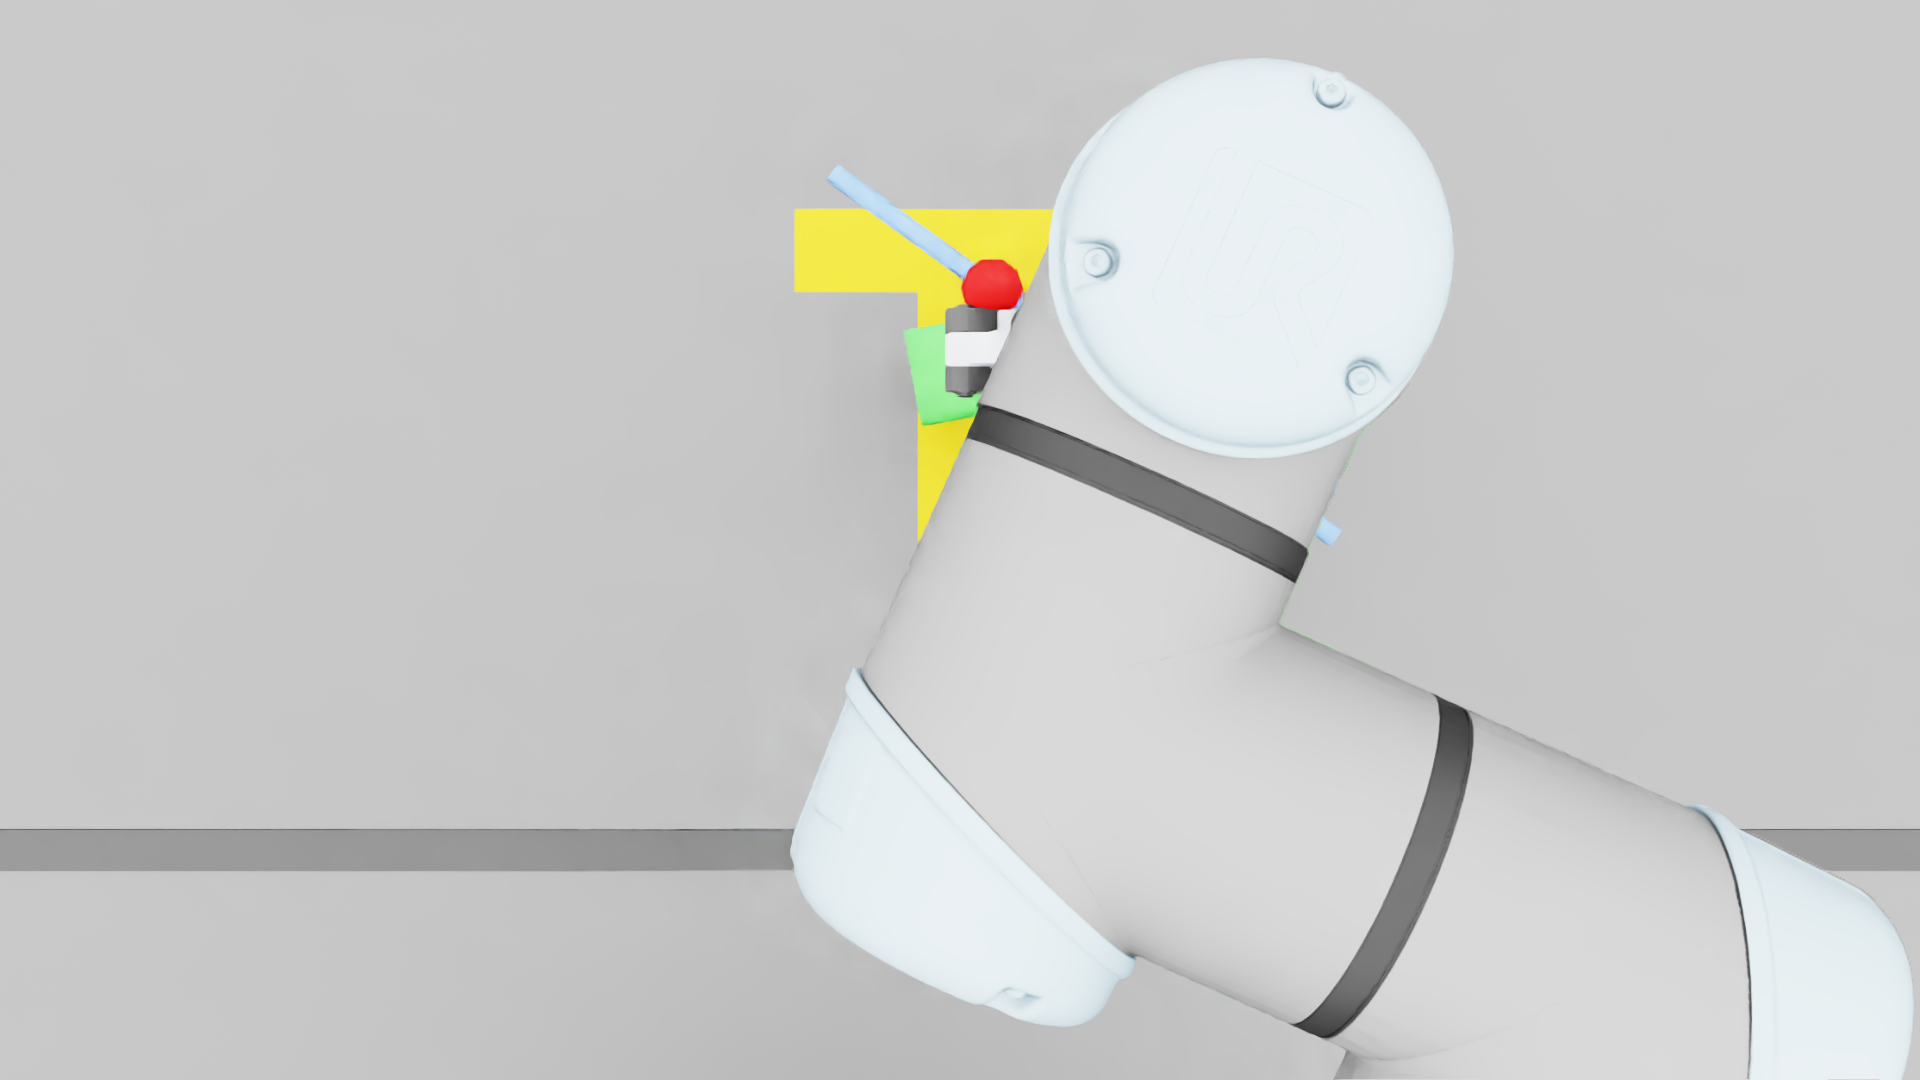
\includegraphics[width=0.32\textwidth]{rec_push_s11_key.png}\hfill
    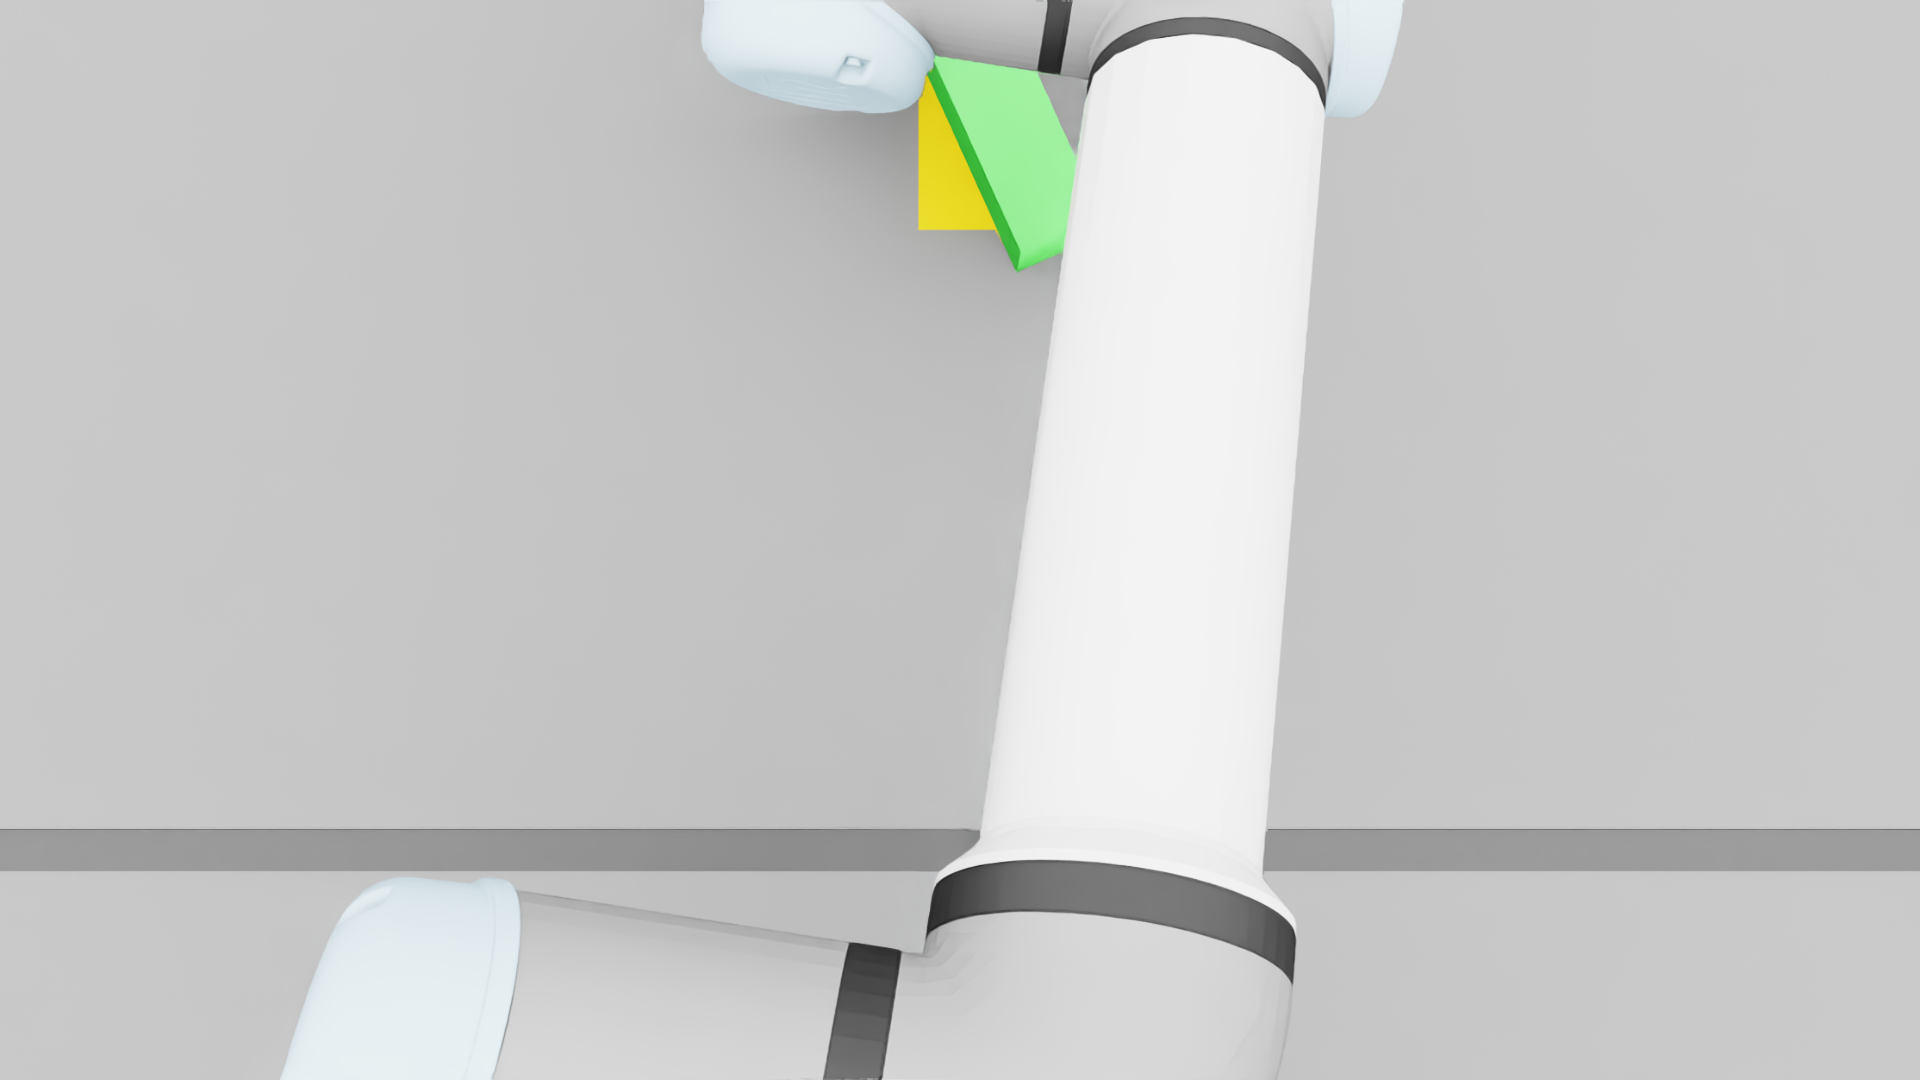
\includegraphics[width=0.32\textwidth]{rec_push_s14_key.png}\hfill
    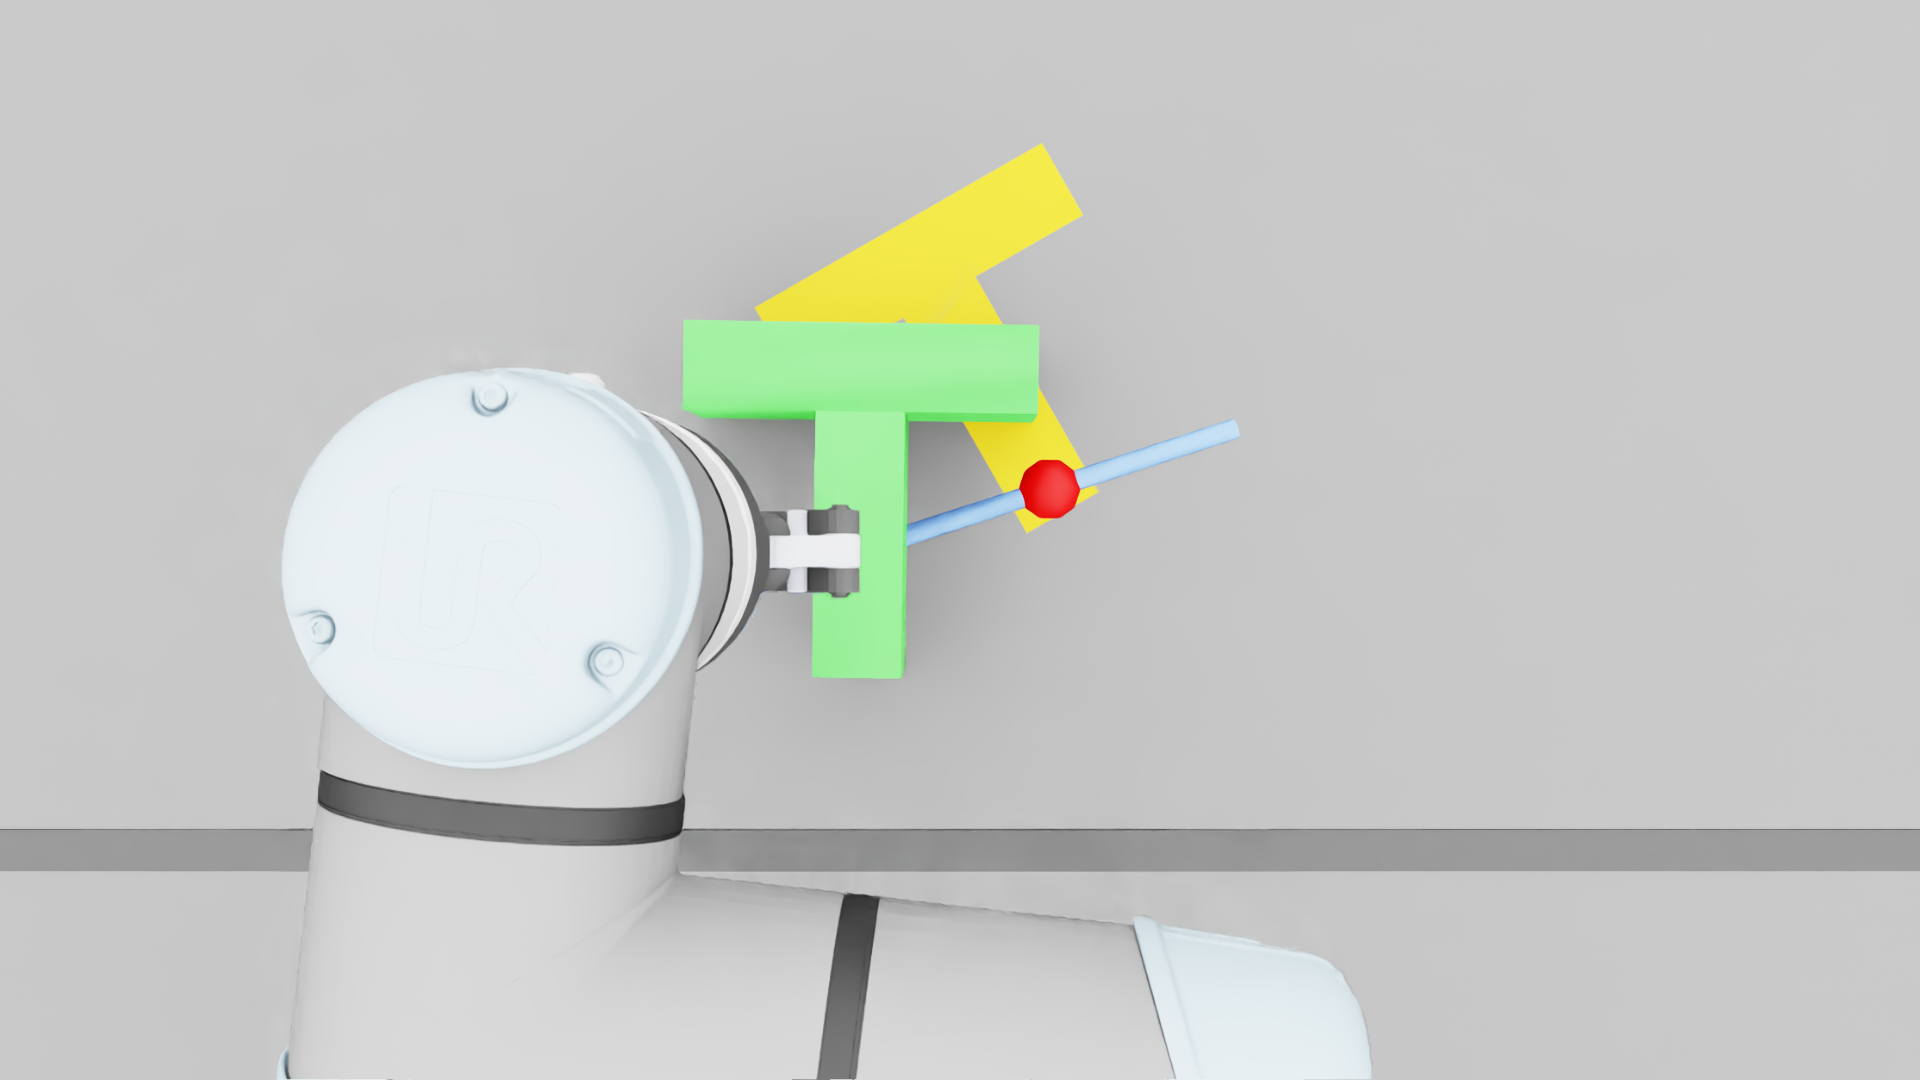
\includegraphics[width=0.32\textwidth]{rec_push_s21_key.png}
    \caption{Keyframes of the single-agent PBRS policy on three held-out scenes.}
    \label{fig:keyframes}
\end{figure}

The off-policy baseline, SAC with Hindsight Experience Replay, did not converge
within the available compute budget. Its status is recorded so that the on-policy
results are read against a concrete off-policy attempt rather than in isolation.
The failure is not evidence against the algorithm family: DDPG with hindsight
experience replay reaches a median success rate of 100\,\% on FetchPush, a
simulated tabletop pushing task, in \cite{Andrychowicz2017}. That published
result serves as plausibility calibration only. The simulator, the object, the
action space, and the compute budget all differ from the present task, so no
success rate is compared directly.


\section{Discussion and Conclusion}
\label{sec:conclusion}

This chapter interprets the results, states the contributions against the three
research questions, records the limitations of the study, and lists directions for
future work.

\subsection{Interpretation}
\label{sec:interpretation}

The central result of this thesis is a priority ordering. For a contact-rich
multi-objective planar-pushing task under a single-GPU budget, effort spent on
principled reward design produces a larger and more reliable improvement than
effort spent on structured training dynamics. The three research questions
decompose this result into an efficiency claim, a comparison claim, and a
mechanistic explanation.

The efficiency claim is direct. Potential-based shaping reduces the parallelism
required for a given success rate by a factor of about four, from 2{,}048 to 528
environments. It also improves the combined-objective success rate by 35
percentage points over the earlier reward at the same gate. The reason was
developed in Section~\ref{sec:pbrs_design}. The potential-based reward is dense,
correctly signed on every push, and bounded, whereas the improvement reward is
negative for most useful pushes and has near-zero variance. The policy-invariance
guarantee of Section~\ref{sec:pbrs} allows this dense signal to be added without
changing the task. The result confirms empirically that the guarantee holds under
stochastic contact physics.

The comparison claim is that neither a forced curriculum nor asymmetric self-play
improves on the plain shaped single-agent model. The curriculum is statistically
equivalent to the single-agent model at the large batch used in Isaac Lab, and
self-play is far worse. This does not contradict the literature that motivates
curricula and self-play; it locates a regime in which they do not pay. The
cross-environment result of Section~\ref{sec:cross_env_results} makes the regime
explicit. The curriculum substitutes for the shaped reward when the batch is small
and gradient estimates are noisy, and adds nothing once the batch is large enough
for stable estimates on both objectives. Reward design and curriculum design are
therefore not independent levers of equal standing. At a sufficient batch size,
the shaped reward already supplies what the curriculum would otherwise provide.

The mechanistic explanation concerns why self-play in particular fails.
Section~\ref{sec:rq3} showed that self-play learns the two constituent skills, each
to roughly 50\,\%, but combines them at about 10\,\%, well below the independence
prediction. Three factors act together to produce this outcome, and all are
specific to this task. First, the physics couples translation and rotation, so the
combined gate cannot be satisfied by treating the objectives separately. Second,
the goal distribution is non-stationary, because the goal-proposing agent changes
it at every iteration, which biases the value term of the GAE advantage as shown
in Section~\ref{sec:pbrs_asp}. Third, the combined gate is strict, so partial
competence on each axis does not accumulate into success. The potential-based
reward supplies enough correctly-signed signal to learn each axis, but it cannot
remove the value-term bias that prevents their composition. This is why shaping
lifts self-play above the near-zero level it reaches under the improvement reward,
yet leaves it far below single-agent training.

\subsection{Relation to Prior Work}
\label{sec:relation}

The findings of this thesis agree with the theory of the papers it builds on,
while qualifying the empirical claims of the papers it tests. The distinction
between the two is worth stating precisely.

On reward shaping, the result confirms \cite{Ng1999PolicyInvariance} under
conditions the original theorem did not examine. Ng, Harada, and Russell proved
policy invariance for finite, discrete Markov Decision Processes with
deterministic dynamics. The present task is continuous, high-dimensional, and
driven by stochastic PhysX contact. The shaping potential is a bounded exponential,
rather than the distance-to-goal heuristics of the original paper. The
potential-based reward reaches the same success rate as the hand-tuned reward
while requiring a quarter of the environments, and never exceeds it. This is the
empirical signature the theorem predicts: shaping changes how quickly the optimal
policy is found, not which policy is optimal. The episodic treatment of
\cite{Grzes2017RewardShaping} licences the undiscounted shaping used here, and the
stable value loss in Appendix~\ref{app:curves} matches the bounded-potential
construction. In this respect the thesis extends an established theoretical result
into a contact-rich robotic regime rather than contesting it.

On asymmetric self-play the relationship is more nuanced, and the negative result
must not be overstated. \cite{Sukhbaatar2018IntrinsicMotivation} demonstrated
self-play in reversible or resettable gridworlds and continuous control tasks,
where the goal is a single state to be reached. \cite{OpenAI2021AsymmetricSF}
scaled it to robotic manipulation with large distributed compute and a continuous
action space. The present study differs from both on three axes that
Sections~\ref{sec:pbrs_asp} and \ref{sec:interpretation} identify as decisive. The
goal is multi-objective with a strict combined gate, not a single reachable state.
The action is a discrete macro-action over a large MultiCategorical space, not a
smooth continuous control. The compute budget is a single Graphical Processing
Unit, not a distributed cluster. The finding is therefore not that self-play is
ineffective. Rather, in this specific setting it does not compose the two learned
skills, and it stays far below single-agent training under a budget realistic for
one laboratory. This framing is consistent with \cite{Berner2019Dota2}, whose
success with competitive self-play required months of training at very large
scale. Through that lens, the modest self-play result here supports rather than
contradicts the observation that self-play is demanding of scale.

The behaviour of the Alice Behavioral Cloning term deserves specific comment. It
connects a design choice in \cite{OpenAI2021AsymmetricSF} to an outcome observed
here. Plappert and colleagues introduced Proximal Policy Optimization-style
clipping on the behavioural-cloning loss (Equation~\ref{eq:abc}), to prevent the
imitation term from producing aggressive policy updates. In their continuous-action
grasping domain, the demonstrated actions of the goal-proposing agent stay close to
the goal-solving agent's policy, so the clipping is rarely active and the imitation
signal flows. In the discrete, contact-rich pushing domain of this thesis, the
goal-proposing agent's unguided pushes lie far from the goal-solving agent's
goal-directed policy. The probability ratio in Equation~\ref{eq:abc} is therefore
extreme, the clip saturates, and the imitation gradient vanishes. The same
mechanism that stabilises imitation in the original setting removes it here. This
is not a flaw in the original formulation. It is a consequence of applying that
formulation to a domain whose action distribution differs sharply from the one it
was designed for. This also explains why the two self-play variants differ only
through Alice's reward, not through the cloning term.

On curriculum learning, the regime-dependence of
Section~\ref{sec:cross_env_results} refines rather than rejects the surveys of
\cite{Narvekar2020} and \cite{Portelas2020ACLSurvey}. Those surveys motivate
curricula primarily for settings where reward is sparse or exploration is hard.
The present result is consistent with that motivation and makes it quantitative.
The forced curriculum contributes substantially when the batch is small and
gradient estimates are noisy: at the small \texttt{gym-pusht} batch it raises scene
success from 10.0\,\% to 50.0\,\%. It contributes nothing once the batch is large
enough for stable estimates on both objectives. A well-shaped dense reward and a
curriculum are therefore partial substitutes, not independent and additive
interventions. The point at which one ceases to add value over the other is
governed by the gradient-variance regime. To the best of the author's knowledge,
this observation is not made explicit in the cited surveys, and it is one of the
more transferable findings of the study.

Finally, the collapse of the symmetric time-based self-play variant to a fail-fast
equilibrium (Appendix~\ref{app:failfast}) is best read through the game-dynamics
analysis of \cite{Letcher2019GameMechanics}. In the symmetric reward, the
goal-solving agent is penalised for the very solve time that rewards the
goal-proposing agent. This defines a near-zero-sum game whose only stable point
under the observed physics is immediate failure. The asymmetric reward of
\cite{Sukhbaatar2018IntrinsicMotivation} incentivises the proposer without
penalising the solver, and so avoids this degenerate equilibrium. The present
study provides a concrete manipulation-domain instance of why that asymmetry is
not incidental but necessary.

\subsection{Contributions Revisited}
\label{sec:contributions}

The contributions stated in Chapter~\ref{sec:introduction} can now be given
quantitative content, one per research question.

For RQ1, the thesis formulates a potential-based reward for multi-objective planar
pushing. It combines bounded exponential position and orientation potentials with
a unified $\mathrm{SE}(2)$ distance. This reward reaches 80.0\,\% scene success at
528 environments, matching the improvement reward at 2{,}048 environments and
improving the combined-objective rate by 35 percentage points.

For RQ2, the thesis provides a controlled comparison of four training regimes
under an identical reward, budget, and evaluation protocol. The forced curriculum
is statistically equivalent to the single-agent model, at 76.7\,\% against
80.0\,\%, a difference that is not significant. Both self-play variants are far
worse, at 16.7\,\% and 6.7\,\%. The cross-environment comparison establishes that
the value of the curriculum depends on the per-update batch size.

For RQ3, the thesis diagnoses the self-play failure by separating per-axis
competence from combined success. Self-play learns each of position and
orientation to roughly 50\,\%, but combines them at about 10\,\%, roughly 2.5 times
below the independence product. The goal-proposing agent, meanwhile, remains a
reliable source of valid goals. This locates the failure in skill composition
under a non-stationary goal distribution, not in skill acquisition.

\subsection{Limitations}
\label{sec:limitations}

Several limitations bound the scope of these conclusions. Validation uses a single
seed per model, so the reported scene success rates carry no confidence intervals.
Only the training-time success rate has variance data, across five chains for the
single-agent model. The best-of-20 protocol raises the scene success rate above
the trial success rate by 14 percentage points for the strongest model. Both
numbers are reported, but the headline figure is the more favourable of the two by
construction. The comparison between self-play and single-agent training differs on
more than one axis at once. These include the number of agents, the goal
distribution, the episode budget, the goal encoder, and the behavioural-cloning
term. The comparison therefore isolates self-play as implemented, rather than the
goal-proposal mechanism alone, and the axes of variation are enumerated in
Appendix~J. The sensitivity of the potential-based reward to its parameters $k_p$,
$k_r$, and $w$ was not systematically tested; the values used were chosen from
pilot runs. Finally, the off-policy SAC with Hindsight Experience Replay baseline
did not converge within the available budget, so the external calibration relies
on published planar-pushing results rather than a converged in-house baseline.

\subsection{Future Work}
\label{sec:future_work}

Each limitation suggests a concrete continuation. Repeating the validation across
multiple seeds would attach confidence intervals to the scene success rates. It
would also place the 3.3-percentage-point single-agent-against-curriculum
difference on a firmer statistical footing. A relaxed or partial-credit success
gate, which rewards satisfying each axis rather than only the conjunction, would
test whether the composition failure can be alleviated by softening the strict
gate. The symmetric time-based self-play variant collapses to a fail-fast
equilibrium (Appendix~\ref{app:failfast}); the zero-sum stability analysis of
\cite{Letcher2019GameMechanics} suggests where a stabilised formulation might be
sought. A systematic sweep of the per-update batch size would map the boundary of
the regime in which the curriculum substitutes for the shaped reward, identified
qualitatively in Section~\ref{sec:cross_env_results}. Completing the SAC with
Hindsight Experience Replay baseline to convergence would supply the off-policy
calibration that the present study leaves open. Finally, transferring the shaped
single-agent policy to a physical UR5e would test whether the efficiency gain
survives the reality gap.

Beyond these direct continuations, the relation to prior work in
Section~\ref{sec:relation} points to two deeper questions. The first is whether
self-play can be made competitive by addressing the specific failure identified,
rather than by adding scale. The value term of the Generalized Advantage
Estimation advantage is biased by the non-stationary goal distribution
(Section~\ref{sec:pbrs_asp}). A goal-proposing agent that changes the distribution
more slowly might keep the value estimate accurate enough for the two skills to
compose. One could constrain the rate of change of the proposed goal distribution,
or train the goal-solving agent against a mixture of current and past proposers.
This would test directly whether the composition failure is intrinsic to
self-play or an artefact of an over-aggressive proposer. The second question
concerns the behavioural-cloning term. The clipping mechanism of
\cite{OpenAI2021AsymmetricSF} removes the imitation signal in the discrete action
space used here. An unclipped or adaptively clipped cloning loss, or one defined
on the decoded continuous push parameters rather than the discrete bins, might
restore the demonstration signal the original formulation relies on. Both
directions treat the negative self-play result not as a dead end, but as a
localisation of where the method breaks in this domain.

\subsection{Conclusion}
\label{sec:final}

This thesis compared reward shaping against structured training dynamics on a
single contact-rich planar-pushing task, under a common budget and a common
success criterion. Potential-based reward shaping reduced the parallel-environment
requirement by a factor of about four and improved combined-objective success by
35 percentage points. A forced curriculum added no value at a sufficient batch
size, and asymmetric self-play performed far worse than single-agent training. The
self-play failure was traced to an inability to combine two individually-learned
skills under a non-stationary goal distribution, not to any failure to learn the
skills themselves. The practical recommendation that follows is simple: invest
first in a principled dense reward, and add structured training dynamics only in
the small-batch regime where they demonstrably contribute.

\pagestyle{contents}

\bibliographystyle{ieeetr}
\bibliography{biblio}

% !TEX root = ../main.tex
\pagestyle{appendix}
\appendix
\section*{Appendices}
\addcontentsline{toc}{section}{Appendices}
\renewcommand{\thesubsection}{\Alph{subsection}}

\subsection{Push Mechanics: Limit Surface and Characteristic Length}
\label{app:mechanics}

The limit-surface normality condition of Equation~\ref{eq:normality} states that
the instantaneous motion twist of a quasi-statically pushed object is normal to
its friction limit surface at the point corresponding to the applied wrench. Its
practical consequence for the task concerns any off-centre push, one whose line of
action does not pass through the object's centre of friction. Such a push produces
a wrench with a non-zero moment component, and therefore a twist that contains an
angular velocity. Almost every push consequently changes both position and
orientation.
The characteristic length $L$ used in the $\mathrm{SE}(2)$ distance of
Equation~\ref{eq:dpose_methods} is the radius of gyration of the object, a
physical constant; for the T-block $L = 0.07\,\text{m}$. It is not a tuning
parameter, and it sets the weight of an orientation error relative to a position
error in a manner consistent with the object's mass distribution. For the
rotationally symmetric disc the characteristic length is set to zero, which
collapses the $\mathrm{SE}(2)$ distance to a pure position distance and encodes the
absence of an orientation objective. The mechanical contrast between the two
objects, the coupled twist of the T-block against the pure translation of the disc,
is discussed in Section~\ref{sec:pushing}.

\begin{figure}[H]
    \centering
    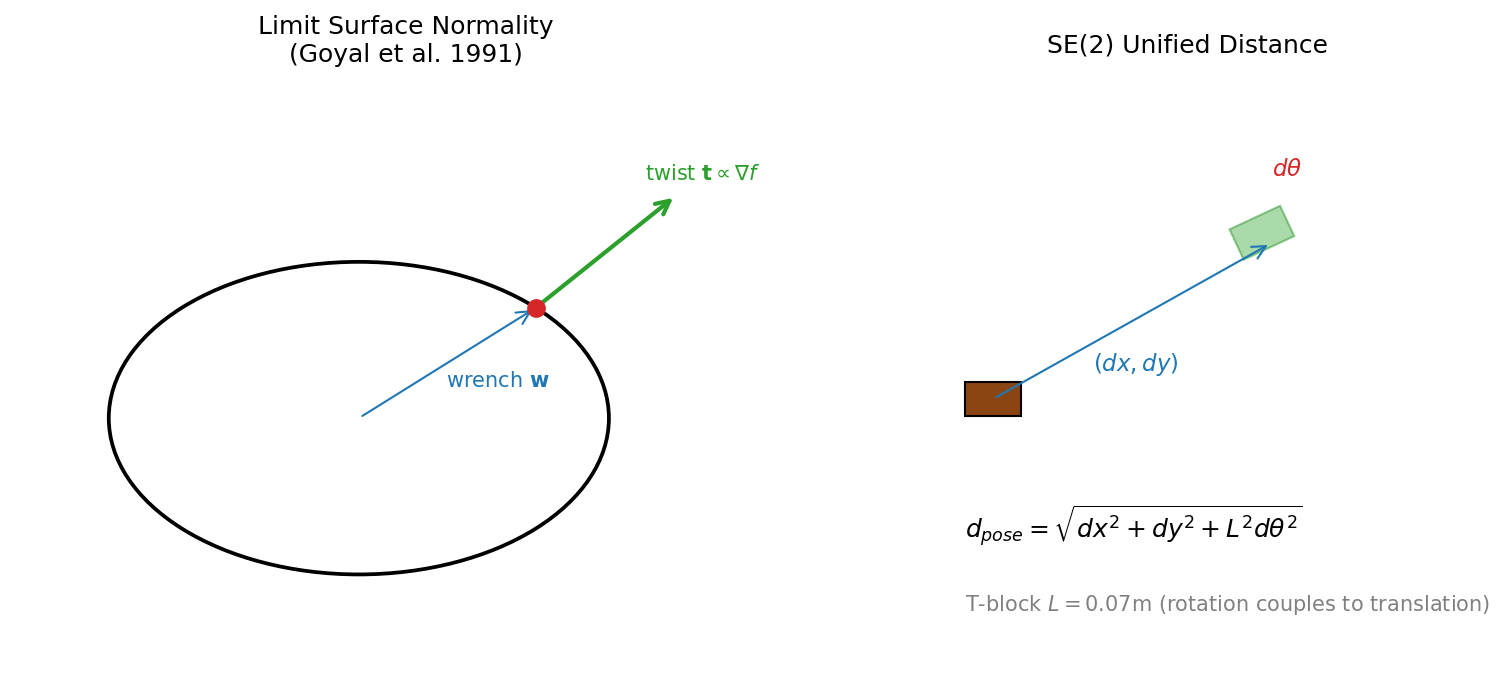
\includegraphics[width=0.6\textwidth]{diagram_limit_surface.png}
    \caption{An off-centre push produces coupled translation and rotation of the
    T-block. The motion twist is normal to the friction limit surface.}
    \label{fig:app_limit_surface}
\end{figure}

\subsection{Training Curves}
\label{app:curves}

Figure~\ref{fig:app_curves} shows the training-time success rate and value loss
for the single-agent and curriculum models. The single-agent model improves
steadily over roughly 3{,}000 iterations, the curriculum model follows a similar
trajectory, and the value loss remains stable throughout, which reflects the
bounded range of the exponential potentials.

\begin{figure}[H]
    \centering
    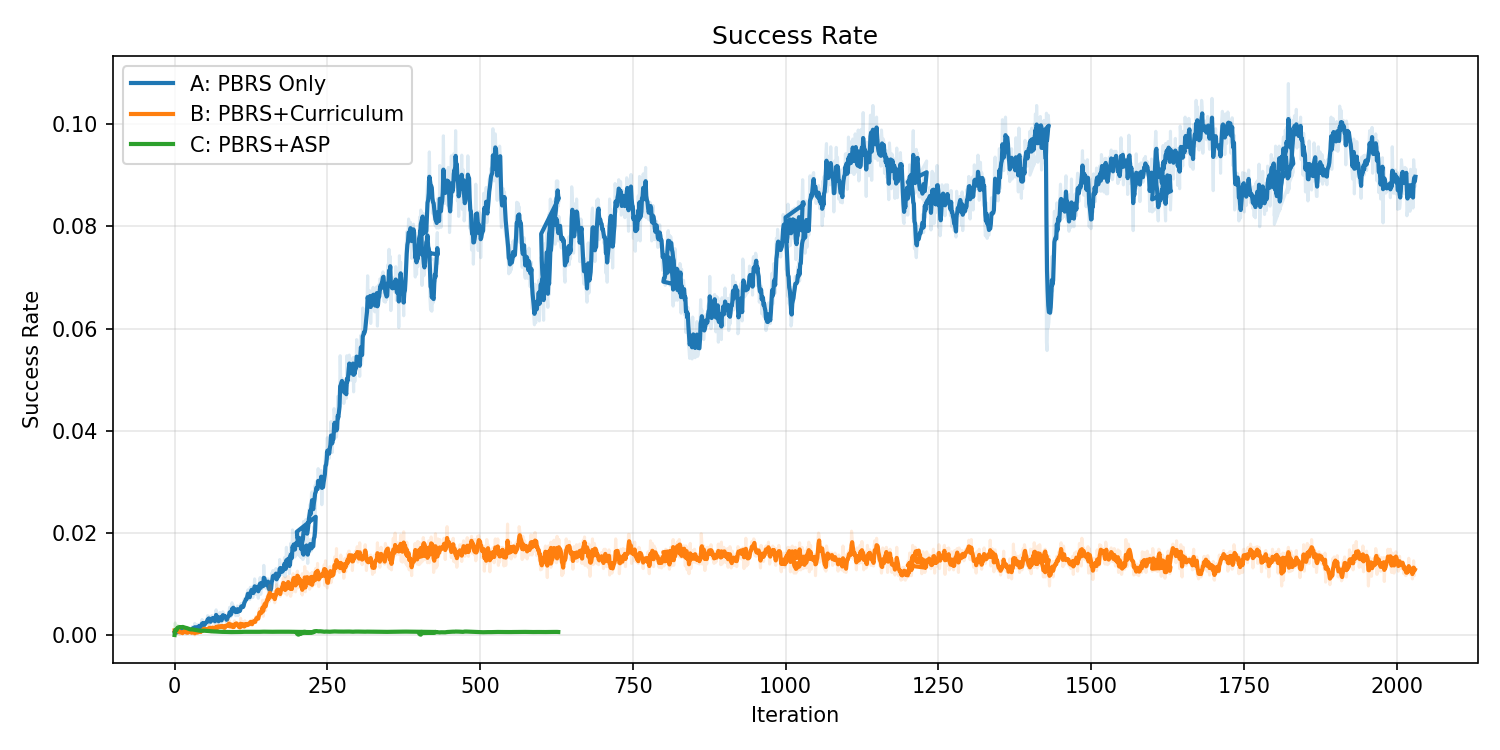
\includegraphics[width=0.48\textwidth]{cmp_Success_Rate.png}\hfill
    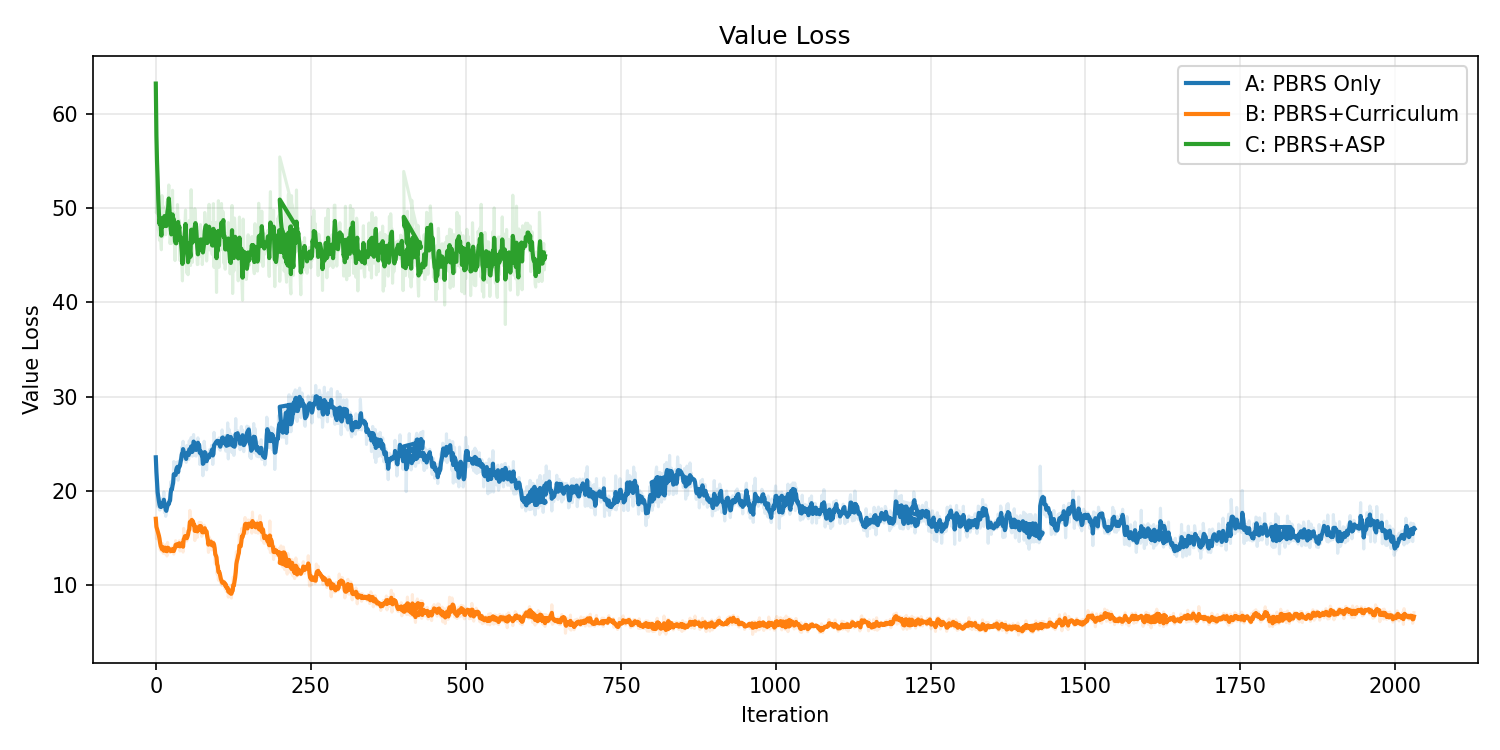
\includegraphics[width=0.48\textwidth]{cmp_Value_Loss.png}
    \caption{Training success rate (left) and value loss (right) for the
    potential-based models.}
    \label{fig:app_curves}
\end{figure}

\subsection{PBRS Parameter Sensitivity}
\label{app:sensitivity}

The potential-based reward uses $k_p = 30$, $k_r = 5$, and $w_{\text{pos}} =
w_{\text{rot}} = 10$, chosen from pilot runs. A systematic grid over these
parameters was not performed within the available budget. The robustness of the
reward to its parameters is therefore not established here. It is recorded as a
limitation in Section~\ref{sec:limitations} and as a direction for future work in
Section~\ref{sec:future_work}. A grid over $k_p \in \{10, 20, 30, 50\}$ and
$w \in \{5, 10, 20\}$, evaluated at the 30-scene gate, would provide the missing
sensitivity analysis.

\subsection{Validation Scene Descriptions}
\label{app:scenes}

The 30-scene held-out suite is defined in \texttt{validation\_configs.py} and
comprises three groups of ten. Scenes 1 to 10 are rotation-dominant, with
orientation changes up to $\pi$ radians and mixed translations. Scenes 11 to 20
are position-only, with the goal orientation equal to the start orientation.
Scenes 21 to 30 combine a position change with an orientation change. Within each
group, difficulty is graded easy, medium, and hard by the start-to-goal distance
and the magnitude of the required rotation. All coordinates are expressed in the
environment-local frame in metres, and orientations in radians.

\subsection{cuRobo IK Pipeline and Workspace}
\label{app:ik}

Each decoded push primitive is executed as a five-phase Cartesian trajectory,
approach, descend, push, retract, and return, spanning 72 physics substeps. Every
waypoint is mapped to arm joint targets by the cuRobo 0.7.5 batched Inverse
Kinematics solver, with the gripper held closed throughout. The reachable
workspace is bounded to the region over the table where the solver returns
elbow-up solutions. Pushes whose start or end points fall outside this region are
clamped to the boundary before execution, so the credit assigned to an action
matches the motion actually performed.

\subsection{Observation Space Specifications}
\label{app:obs}

The single-agent models use a 28-dimensional observation: end-effector pose (6),
object pose and velocity (14), goal pose (6), and the position and orientation
errors (2). The goal-solving agent in the self-play models uses the same
28-dimensional layout, with the goal encoded through the GoalEncoder into an
eight-dimensional latent in the difference variant. The goal-proposing agent uses
a 20-dimensional observation that omits the goal, since it sets the goal rather
than solving it.

\subsection{Confounded Ablation Disaggregation}
\label{app:confound}

The single-agent and self-play models differ on at least eight dimensions at once:
the number of agents (one against two), the goal distribution (fixed random
against adversarial and shifting), the goal encoder (absent against present), the
behavioural-cloning term (absent against present), the historical opponent pool
(absent against present), the rollout length (15 pushes for one agent, against
5 plus 10 split between two), the episode budget (5 pushes for the single agent
against 10 for the goal-solver), and the number of policy updates per iteration
(one
against two). The comparison in this thesis therefore isolates self-play as a
package rather than any single mechanism within it. Four single-dimension
isolations are provided nonetheless: the disc contrast of
Section~\ref{sec:rq2_coupling}, the two Alice reward formulations of
Section~\ref{sec:rq2_reward}, the imitation ablations of
Section~\ref{sec:rq2_abc}, and the goal-encoder ablation of
Section~\ref{sec:rq2_encoder}. The cleanest of these is the reward-formulation
pair, whose members differ only in the goal-proposing agent's reward. It shows no
consistent advantage for either formulation. At 528 environments the
outcome-based variant logs a per-push training rate of 35.8\,\%
($\pm$ 8.8\,pp, 5 seeds) against 32.6\,\% ($\pm$ 0.4\,pp, 5 seeds) for the
time-based variant on the T-block, and both transfer zero held-out scenes. On the
disc the time-based variant leads during training (83.8\,\% against 77.9\,\%
per push,
5 seeds each) yet trails slightly on held-out scenes (6.7\,\% against
7.3\,\%).

\subsection{Training Budget Comparison}
\label{app:budget}

Every Isaac Lab run in the experiment set is budget-matched. The total experience
is held at about 23.8 million pushes, and the iteration count is set inversely
proportional to the number of parallel environments. A sweep therefore changes
the per-update batch size alone. The confound that a larger batch also means
fewer gradient updates is stated wherever a scale result appears. The headline
models
train at 528 environments for approximately 3{,}000 iterations. The
potential-based agent and the improvement-reward baseline are additionally swept
across 256 to 2{,}048 environments, and the two self-play subjects across 256 and
2{,}048. At the 528-environment baseline the potential-based single-agent model
reaches a held-out scene success rate of 79.3\,\% ($\pm$ 3.5\,pp, 5 seeds), and
the curriculum model 80.0\,\% ($\pm$ 4.1\,pp, 5 seeds). The improvement-reward
baseline, trained at up to 2{,}048 environments, is still training at the time
of writing; its held-out validation is \TBD, and until it completes the
environment-efficiency comparison between the two reward families remains open.

\subsection{Secondary Variants}
\label{app:secondary}

The two disc self-play models and the Bob-penalty model are headline subjects,
reported in Table~\ref{tab:main_results} and Sections~\ref{sec:rq1} and
\ref{sec:rq2_coupling}; they are not repeated here. The ablation arms, with the
imitation term removed, with the goal encoder removed, and the disc positive
control, appear in Sections~\ref{sec:rq2_abc} and \ref{sec:rq2_encoder}. Two
groups remain outside the main text. The first is the original, non-simplified
potential formulation at the position-only gate. The second is the
cross-environment set: the single-agent, curriculum, and self-play models
retrained in \texttt{gym-pusht}, one seed each, which solve 3.3\,\%, 9.0\,\%,
and 1.0\,\% of the held-out scenes respectively. Both groups are consistent with
the principal findings: self-play remains far below single-agent training across
every variant.


\end{document}